\documentclass[bsc,frontabs,singlespacing,parskip,deptreport]{infthesis}
%Juntar a document class na primeira linha "twoside" para fazer double sided.



\usepackage{pdfpages}
\usepackage[utf8]{inputenc}
\usepackage{float}
\usepackage{url}
\usepackage{tikz}
\usepackage{calc}
\usepackage{ifthen}
\usepackage{pgf-pie}
\usepackage{graphicx}
\usepackage{verbatim}
\usepackage{natbib}
\usepackage{color,soul}
\usepackage{verbatim}
\usepackage{caption}
\usepackage{hyperref}
\usepackage{siunitx}
\usepackage{subcaption}



\hypersetup{
    colorlinks=false,
    linktoc=all
}



\begin{document}


\title{Sensing Spaces: An online spatio-temporal model for PM2.5 predictions using a combination of stationary and mobile airborne particulate sensors}
%\title{\vspace{-5.0cm} \centering{
\includegraphics[scale=0.5]{eushield.eps}} \\ Sensing Spaces: A Study in Mapping Air Pollution in Public Spaces using Personal Exposure Monitors}
\author{Jo\~{a}o Catarino Carvalheiro \break Neto dos Santos}

\course{Master of Informatics}
\project{{\bf MInf Project (Part I) Report}}

\date{\today}

\abstract{
Air pollution monitoring and prediction at an intra-urban scale provide important information at the individual and community level. 
This project proposes an online spatio-temporal model that predicts $PM_{2.5}$ concentrations in space and time, using a combination of mobile sensor data and stationary sensor data collected by AIRSpeck sensors. The model can be trained and make predictions in a real-time context. The model uses Ordinary Kriging and Passive-Aggressive Regressors and was tested on mobile data of two datasets provided, collected in the central area of Edinburgh in July 2018. The model performs better when mobile data is used in conjunction with stationary data. With both types of data, it performed 19\% better than the baseline. Error correction algorithms were compared on the second dataset. The best method found uses a median of global errors with at least three past observations, and this correction further improved results by 22\% compared to the base model, having an MAE of 0.948. 
Improvements were made to the existing user interface of the Android application for the AIRSpeck-P and RESpeck data collection, to add media collection functionality and it was tested by ten participants using the sensors.


%Proved that the use of mobile data in the training process improves results.
%Error correction also improves results.
}

\maketitle

\section*{Acknowledgements}
A word of gratitude and appreciation to my supervisor Professor D.K. Arvind, for his proposal, guidance and support throughout the project. 

Thank you to Ivan Angelinin, Mantas Miksys and Zo\"e Petard for their previous work on the Sensing Spaces project, and the participants that volunteered to test part of this work.

To my father and mother for all their unconditional support and encouragement, and Santiago Garcia for his companionship.

\tableofcontents

%\pagenumbering{arabic}

\chapter{Introduction}
Air pollution causes harm to humans but also other living organisms and may damage the natural and anthropogenic environment. Breathing polluted air can trigger respiratory problems, such as asthma, aggravate health conditions or even cause cancer, lung diseases, brain and nerve damage \cite{epa}.

The society, environmental agencies and governments demonstrate concern about air quality and are actively promoting a cleaner, healthier air in their regions, for example with the application of legislation. The United States Environmental Protection Agency, as an example, produced the Clear Air Act \cite{epa} to control and regulate the production of pollutants in the atmosphere.

Accurate monitoring and prediction is essential to inform and enforce goals established by local authorities. Its importance to policymakers also extends to economic benefits, as high pollution levels incur in costs, for example, increased health costs \cite{zoe}.

In the community and individual level, high-resolution information about air pollution allows citizens to make better decisions regarding commuting around the city or deciding where to spend their time outdoors. Besides, vulnerable people such as people with respiratory diseases can be warned of future short-term pollution peaks that might affect their condition, allowing them to avoid or prepare to minimise risk.

Usually, air quality is monitored by networks of static air quality monitoring stations operated by local city authorities to comply with the statutory requirements for air quality levels. Although these types of equipment are expensive and have to be calibrated at regular intervals, they are accurate and provide detailed results on suspended particulate and gaseous pollutions. However, this means the quantity is limited, and intra-urban environments cannot be studied. 


The AIRSpeck and RESpeck sensors were developed by the Center of Speckled Computing at The University of Edinburgh. The AIRSpeck sensors have a stationary and a mobile form factor, allowing to be either mounted to street furniture or worn as a belt. They measure air quality, including $PM_1$, $PM_{2.5}$ and $PM_{10}$ and are much smaller and cheaper than conventional air monitoring stations. The RESpeck sensor is a respiratory monitor that is worn as a plaster on the chest and collects breathing information such as breathing rate. More information about these sensors is presented in the Background chapter.

Using the AIRSpeck sensors allow for a greater quantity of sensors to be deployed which also allows a higher spatial resolution study of air pollution phenomena. These form a network of sensors collecting data at different times and places and enable an intra-urban analysis, which is not possible with the few reference air quality monitors in a city.

Previous work in the Sensing Spaces project has also focused on air pollution predictions and its applications to citizens. Both spatial and temporal models have been studied and, online methods have been researched, providing evidence that machine learning is a useful technique for air pollution prediction in general. Also, work to visualise, collect and apply this data in a useful and straightforward manner has been developed. Examples of such applications are web interfaces for visualisation of pollution data, android applications that communicate with the sensors for more accessible data collection and path planning algorithms to improve citizen's paths and reduce their exposure to particulate matter. Previous work is described and analysed in detail in the Literature Survey chapter.

The primary goal of the project is to produce an online spatio-temporal model that uses a combination of data from static sensors and data from mobile sensors to predict $PM_{2.5}$ levels in the future. Such a model should make better predictions, compared to the stationary-only case, due to the greater quantity of data and the ability to adapt the model. However, implementing such a model is challenging due to the sparsity of the mobile data and its unpredictability as to when and where we will get this data.

The model proposed uses a spatial and an online temporal model, Ordinary Kriging and Passive-Aggressive Regressor respectively. These are used to interpolate predictions in space and time. This project uses a well-defined area in Edinburgh where data was collected, and predictions were performed. The produced model is online as it learns over time and adapts to changing circumstances, spatial because it can interpolate to regions where observations did not occur and, lastly, temporal as it is able to make predictions into the future.

Such model needs to be compared to other baselines; therefore the implementations of those baselines and the comparison with the model and analysis of the results is also essential for this project and is detailed in the Methodology chapter. 

The model performs better than the baselines, both established and defined by previous work. Moreover, several error correction techniques were also tested, and they were used to prevent the model from underpredicting and to learn using past errors made continuously. This technique improved the results of the model further.

The Android application that connects to the sensors to collect data was also improved to allow users to collect qualitative data in the form of media. The User Interface was enhanced to include new buttons that integrate into the existing application.

\section{Main Contributions}

An improved User Interface was developed for the AIRSpeck android application to allow media collection by the users including photographs, video, text and audio clips. The application and sensors were tested by ten participants and results were collected, visualised and analysed.

For the model, an external dataset was used, so it was visualised, calibrated and outliers were removed. The temporal prediction model was optimised, and its integration with the spatial interpolation method was implemented. The performance of the model was continuously evaluated and compared to different baselines, both newly created and reported in previous work.
The spatio-temporal model performs predictions in space and time dimensions, and the model performed significantly better than baseline and was further improved with an error correction technique. The online characteristic of the model allows a possible real-time deployment of the system, not only predicting in real time but also adapting and training in real time.

The novel contribution of this work is for the first time an online spatio-temporal model has been created using a combination of an online temporal prediction model and spatial interpolation model to predict $PM_{2.5}$ values in high resolution ($48m \times 48m$). It is also the first time that mobile data is used in the training part of the model, improving the performance of the model, instead of just using mobile data as validation of the algorithm.

\section{Report Structure}

In Chapter 2 the background of air pollution, particulate matter, information about the sensors and online machine learning is introduced.

Chapter 3 describes the literature review performed on previous projects on the Sensing Spaces project and other relevant literature.

Chapter 4 describes the development of an improved user interface for the AIRSpeck mobile app and the results of the tests on study participants.

Chapter 5 gives more detail about the methodology, the model proposed, how it works and the justification for the choices made.

In Chapter 6 the results and discussion about the model's behaviour are explained as well as different performance comparisons with baselines.

Lastly, Chapter 7 is a summary of the report and indicates future improvements and the next phases for Part 2 of the MInf project.


\chapter{Background}
\section{Air Pollution and Particulate Matter}

Air pollution has an impact on the health of communities and individuals, such as cardiovascular and respiratory diseases, strokes and cancers \cite{scor}. According to the World Health Organization (WHO) \cite{whofactsheet}, "more and more, evidence demonstrating the linkages between ambient air pollution and the cardiovascular disease risk is becoming available". Air pollution sources can be anthropological, such as burning fossil fuels, agriculture and waste treatment or they can be natural sources such as volcanic eruptions, forest fires and sand storms \cite{signals}.

Particulate Matter (PM) is a mixture of solid and liquid particles found in the air. Some of them are not visible with the naked eye and are absorbed by our lungs when inhaled. PM is measured in micrograms per cubic meter ($\mu g m^{-3}$) and can have several size filters: $PM_{10}$ which includes particles which are $10\mu m$ or smaller, $PM_{2.5}$ which includes particles which are $2.5\mu m$ or smaller and  $PM_1$ which includes particles smaller than $1\mu m$.

Exposure to PM2.5, in particular, has been studied to have a negative impact on people's health and was attributed the fifth-ranking mortality risk factor in 2015 \cite{lancet}.

The World Health Organization Air Quality Guidelines state that fine particulate matter (PM2.5) should not exceed 10 $\mu g/m^3$ annual mean and 25 $\mu g/m^3$ 24-hour mean and coarse particulate matter (PM10) should not exceed 20 $\mu g/m^3$ annual mean and 50 $\mu g/m^3$ 24-hour mean \cite{whofactsheet}. The same organisation reports that ambient air pollution was estimated to cause 4.2 million premature deaths in 2016 worldwide due to exposure to PM2.5, 91\% of those in low- and middle-income countries, especially in the South-East Asia and Western Pacific regions \cite{whofactsheet}. WHO is deeply committed to responding to the adverse health effects of air pollution. 


\section{AIRSpeck and RESpeck sensors}

The RESpeck sensor (Figure \ref{fig:e}) is a respiratory monitor that includes a 3-axis gyroscope and accelerometer that is worn as a plaster on the chest, as observable in Figure \ref{fig:f}. It allows tracking respiratory movements such as breathing rate and other breathing properties \cite{estimation_dosage}. 

The AIRSpeck family of sensors \cite{airspeck_family} is comprised of two sensors: the AIRSpeck-S (Stationary) and the AIRSpeck-P (Personal), the latter often referred to as mobile sensor in this project, given its wearable usability. The AIRSpeck-S, observable in Figure \ref{fig:b} is a portable stationary sensor that can be attached to street furniture and measure temperature, humidity, $PM_1$, $PM_{2.5}$, $PM_{10}$, nitrogen dioxide ($NO_2$) and ozone ($O_3$) concentrations. The sensor components are listed in Figure \ref{fig:a}. The PM values are derived from an Optical Particle Counter that classifies particles by size between $0.38\mu m$ and $17 \mu m$ into 16 different categorised bins. Data from AIRSpeck-S sensors are sent to a server through the GSM network using a GPRS module. The AIRSpeck-P sensor provides similar functionality in a different form factor (Figure \ref{fig:c}). It includes a battery and can be worn as a belt (Figure \ref{fig:d}) or sash and be used to monitor personal exposure of pedestrians. AIRSpeck-S sensors collect data every 5 minutes, while AIRSpeck-P sensors collect at a higher rate of 10 seconds.

The AIRSpeck family of sensors and RESpeck sensor were developed by the Centre for Speckled Computing at the University of Edinburgh. Both types of sensor communicate via Bluetooth with an Android application that stores the information collected from sensors and other information such as GPS coordinates and device battery levels \cite{clinical_trials}. Their lower cost, when compared to other high-end systems, high accuracy and high-cost sensors, allow an implementation of a network of these sensors for recording higher amounts of data both in space and in time.

The AIRSpeck sensors use Alphasense OPC-N2 sensor for measuring PM concentrations. In the Particle Counter's User Manual \cite{alphasense}, using the European standard definition of $PM_1$ and $PM_{10}$, the sensor assumes "a negligible contribution from particles below (...) the lower limit of particle detection of the OPC-N2 sensor" and "PM10 extends to particle sizes beyond the upper measurable size limit of the OPC-N2. In some cases, this can result in the reported PM10 value being underestimated by up to ~10\%". Given the possibility of $PM_1$ and $PM_{10}$ measurements having less precision than $PM_{2.5}$ in a low pollution environment such as the city of Edinburgh, and the fact that $PM_{2.5}$ has been proven to have a negative impact on people's health, this project focused on $PM_{2.5}$. However, this model can be applied to other PM values and possibly other pollution metrics such as ozone or nitrogen dioxide concentrations.


\begin{figure}[H]
\centering
\begin{subfigure}{0.48\textwidth}
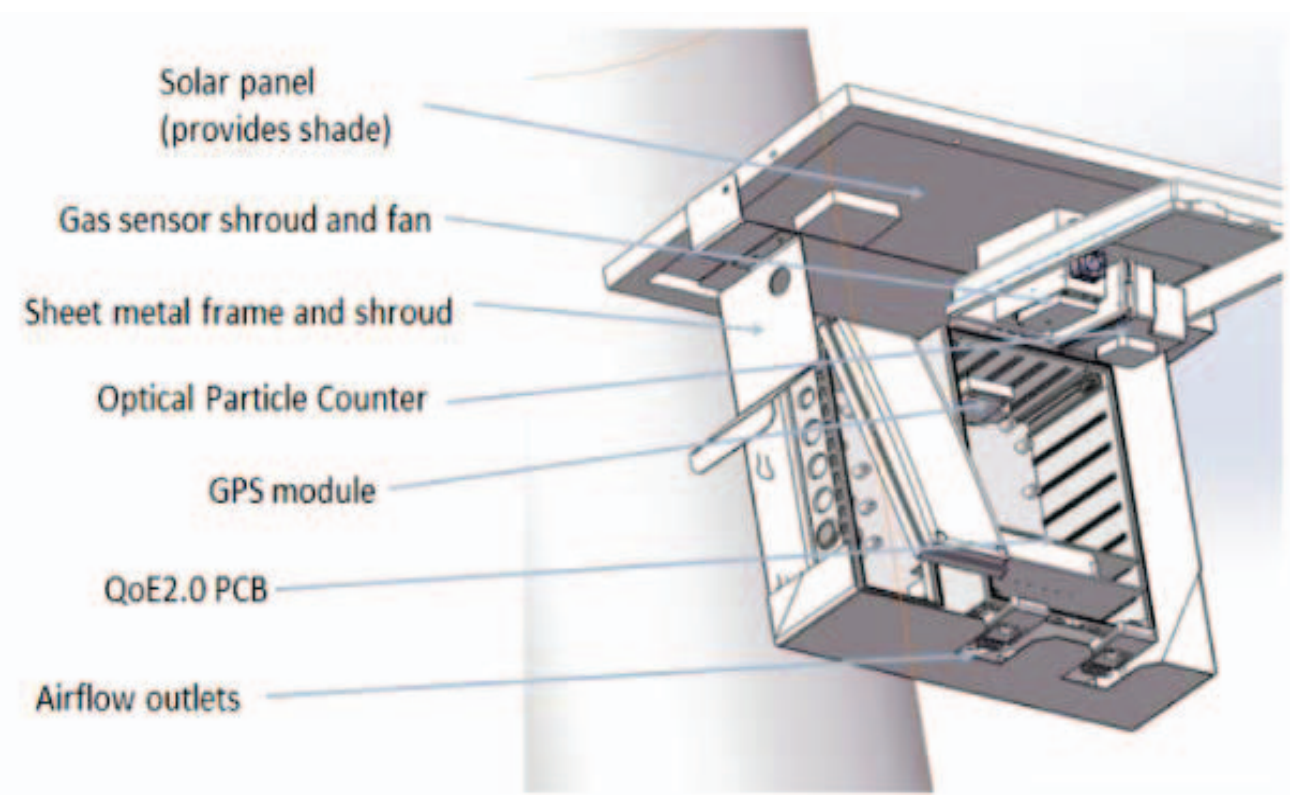
\includegraphics[width=\linewidth]{images/Airspeck_P_inside.png}
\caption{AIRSpeck S composition \cite{clinical_trials}} \label{fig:a}
\end{subfigure}
\begin{subfigure}{0.48\textwidth}
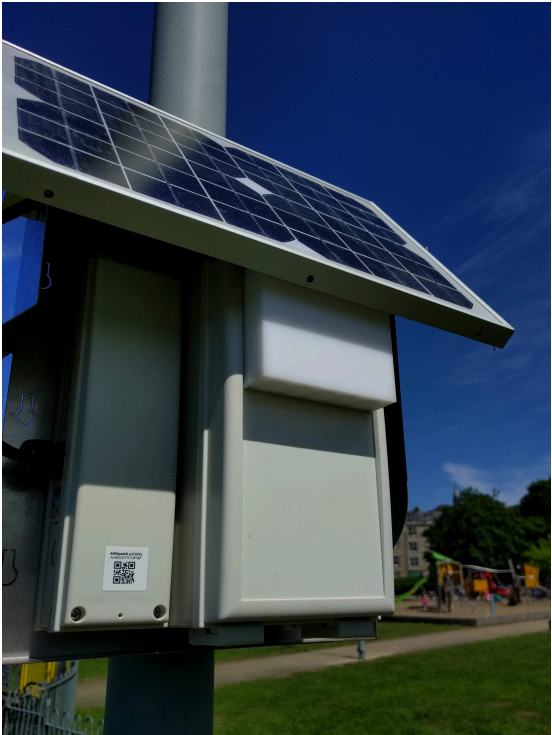
\includegraphics[width=\linewidth]{images/AirspeckS.png}
\caption{AIRspeck S sensor \cite{zoe}} \label{fig:b}
\end{subfigure}

\medskip


\begin{subfigure}{0.48\textwidth}
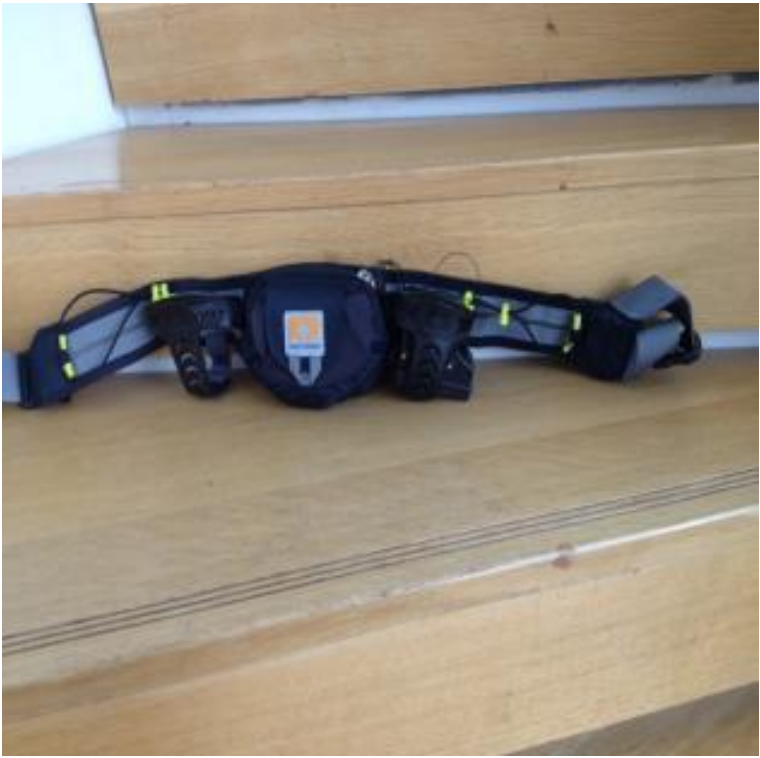
\includegraphics[width=\linewidth]{images/AIRSpeckP.png}
\caption{AIRSpeck P sensor belt \cite{estimation_dosage}} \label{fig:c}
\end{subfigure}
\begin{subfigure}{0.48\textwidth}
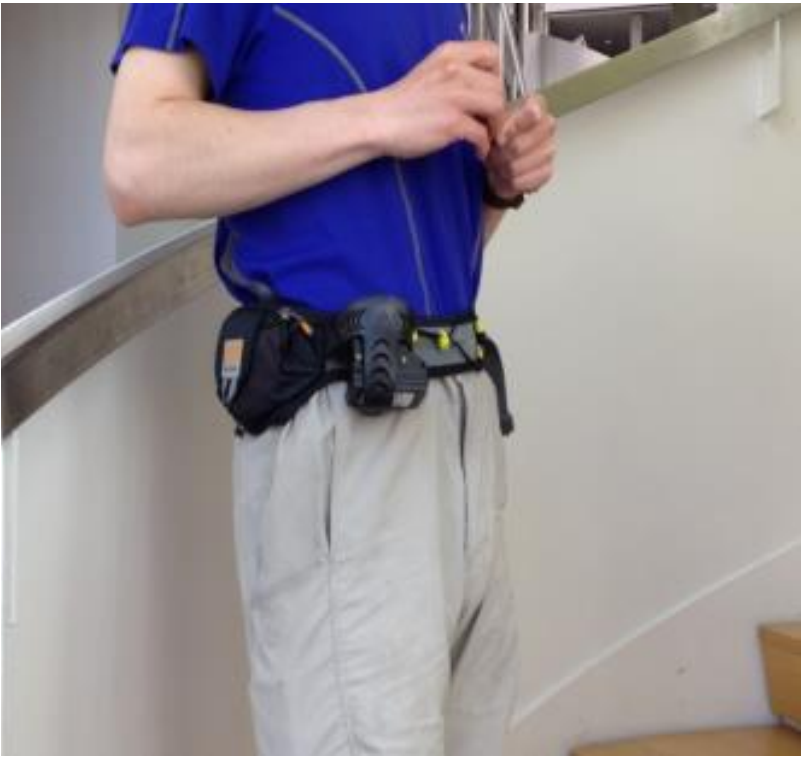
\includegraphics[width=\linewidth]{images/AIRSpeck_P_worn.png}
\caption{AIRSpeck P sensor worn \cite{estimation_dosage}} \label{fig:d}
\end{subfigure}

\medskip

\begin{subfigure}{0.48\textwidth}
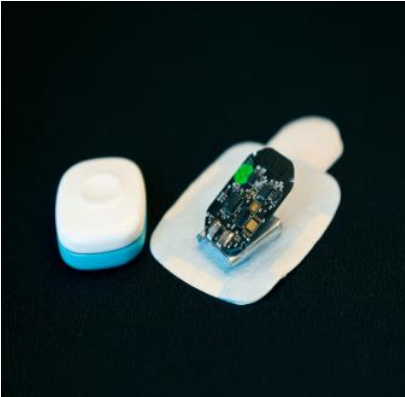
\includegraphics[width=\linewidth]{images/RESpeck.png}
\caption{RESpeck sensor \cite{estimation_dosage}} \label{fig:e}
\end{subfigure}
\begin{subfigure}{0.48\textwidth}
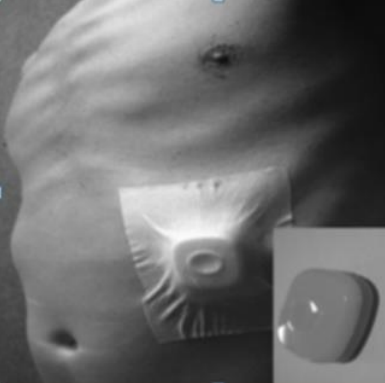
\includegraphics[width=\linewidth]{images/RESpeck_worn.png}
\caption{RESpeck sensor worn on body \cite{estimation_dosage}} \label{fig:f}
\end{subfigure}

\caption{AIRspeck and RESpeck sensors}
\label{fig:sensors}
\end{figure}



\section{Online Machine Learning}
The batch learning method is one of the most commonly used machine learning techniques, also referred to as offline techniques. In batch learning, the best predictor is generated using the entire dataset at once. On the other hand, in online techniques, data becomes available in sequential order and the model updates at each step when data becomes available. Not only an online algorithm makes predictions in real time, but it also trains in real time. This difference in paradigm to "learn" the best predictor can be observed by comparing Figure \ref{fig:batch} and \ref{fig:online}. The online model works in "rounds": at the beginning of each round, an input sample is presented and a prediction is performed. The algorithm verifies if the prediction was good or not and adjust its parameters to fit the prediction better next time. These rounds occur continuously in real time.

Online learning is used for datasets that are infeasible to train on the entire dataset due to their size, for time series data or when it is necessary to adapt to new patterns of data as they come in. This description fits a real-time application of an air pollution prediction model as the data can be quite dynamic and the prediction outcome could depend on a number of external factors such as the weather, traffic patterns and long-range pollution transportation.

Applications of online learning include experiments with social network data, ad placement, dynamic pricing, email categorisation, speech-to-text and music-to-score alignment \cite{mit_course}\cite{applications}.

\begin{figure}[H]
\centering
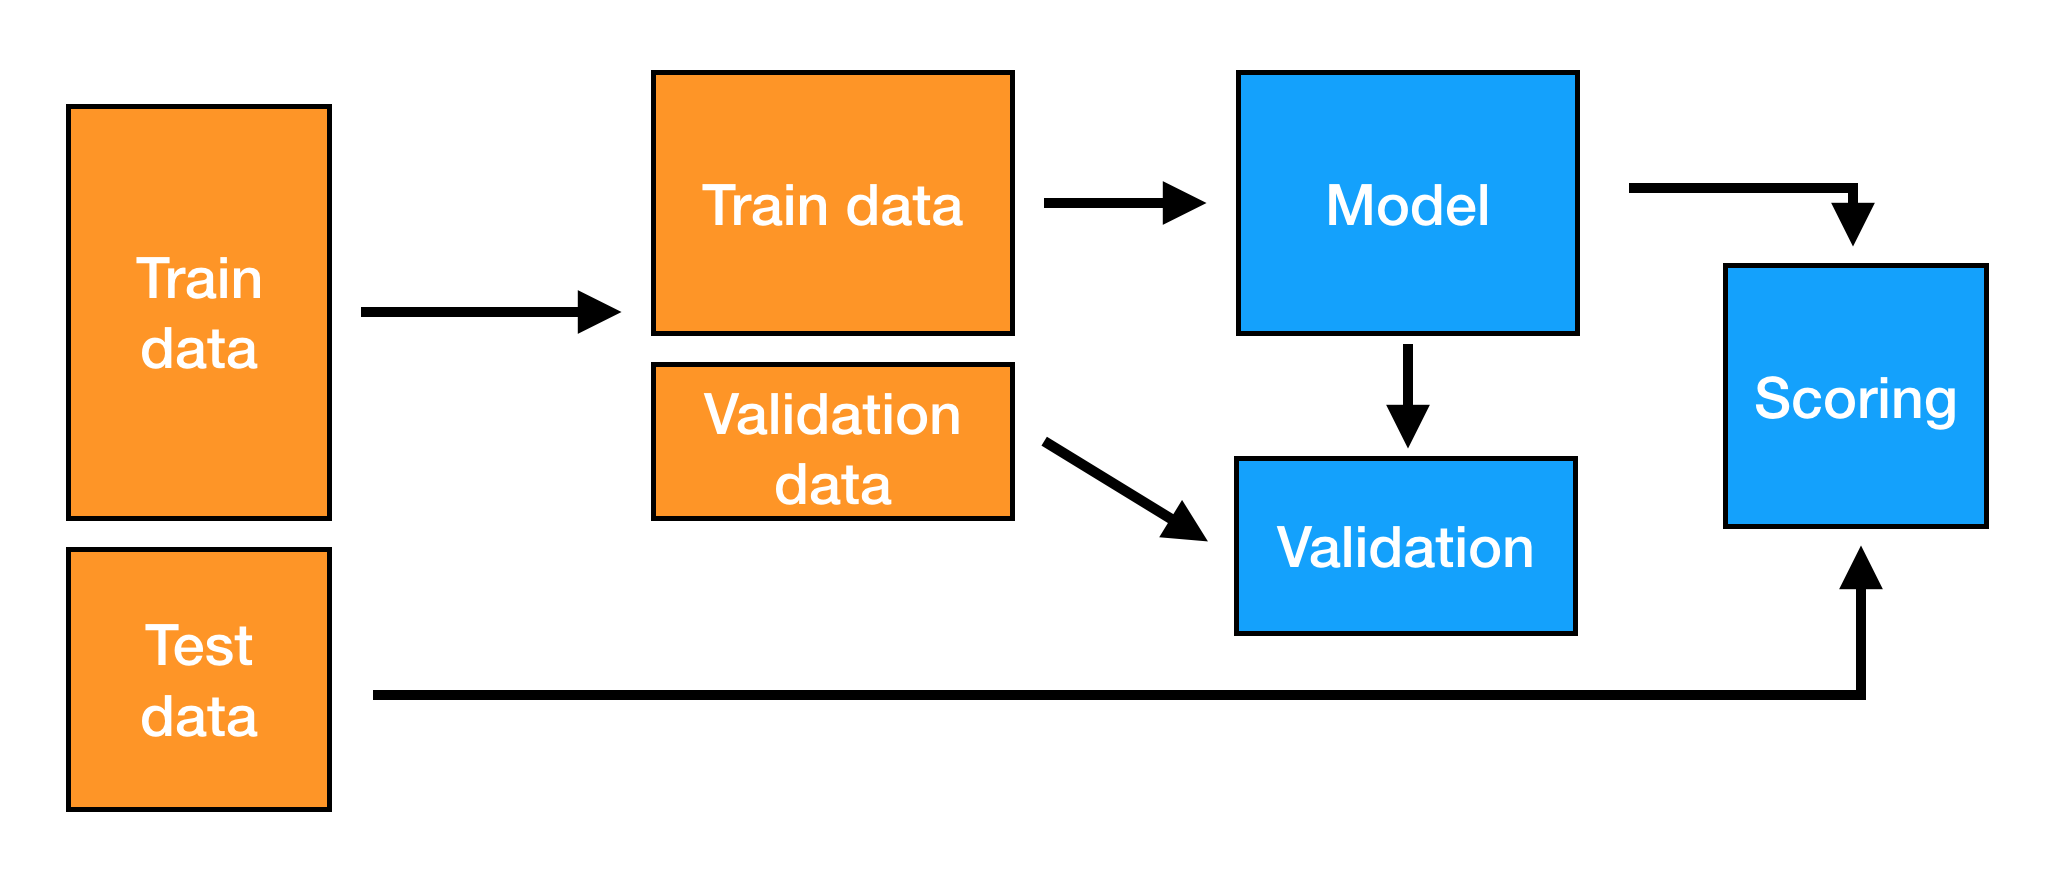
\includegraphics[width=.9\textwidth]{images/batch_learning.png}
\caption{Batch learning model (Offline learning)} \label{fig:batch}
\end{figure}

\begin{figure}[H]
\centering
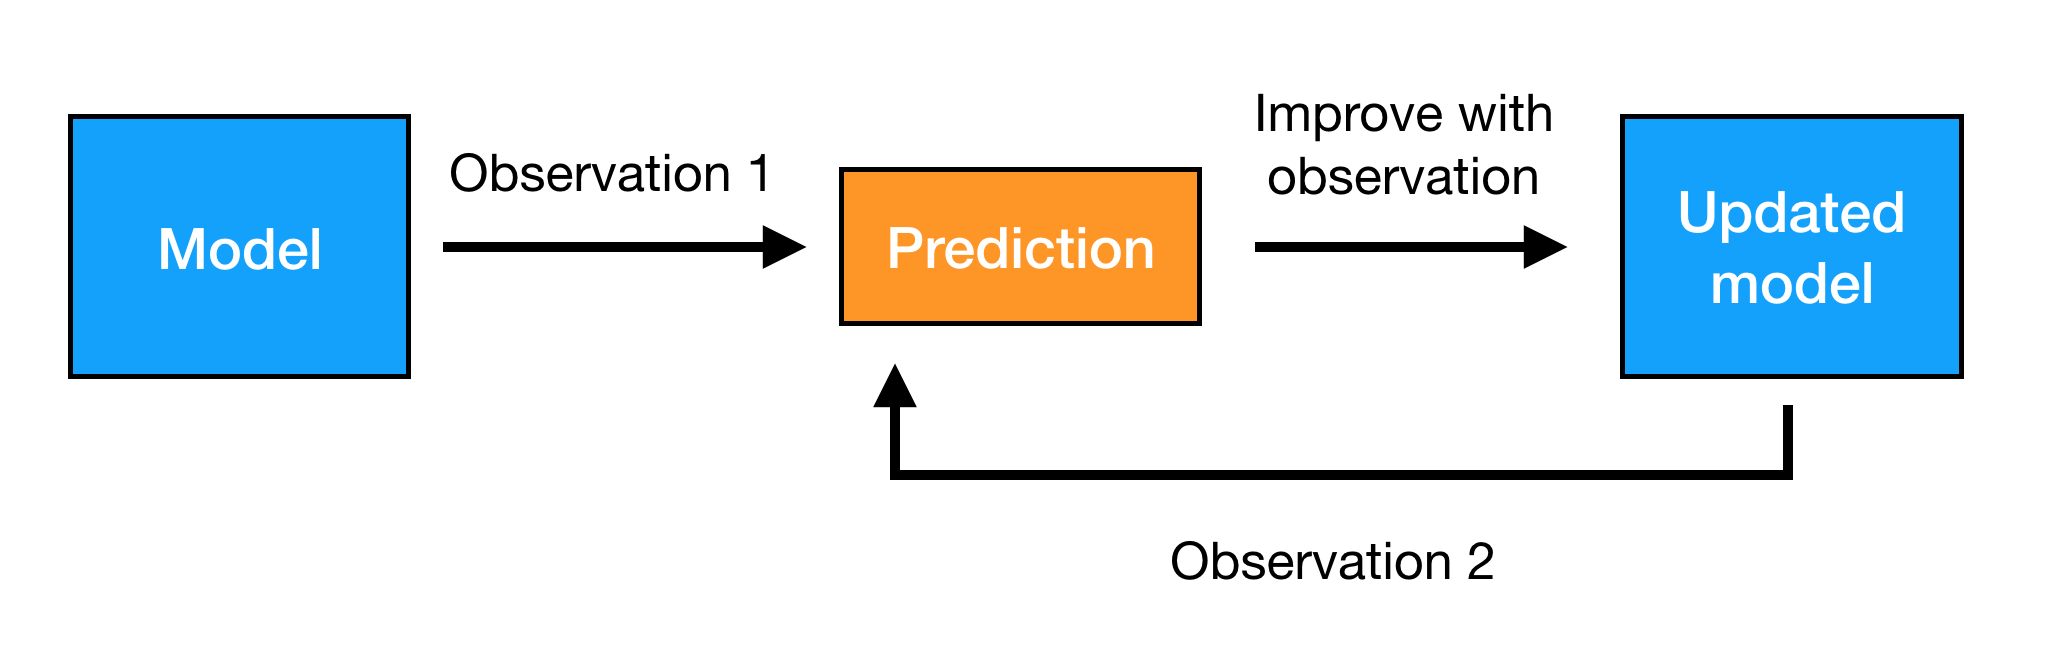
\includegraphics[width=.9\textwidth]{images/online_learning.png}
\caption{Online learning model} \label{fig:online}
\end{figure}





\chapter{Literature survey}
\section{Previous Work}

The Sensing Spaces project is an umbrella term for several problems related to air pollution in public spaces. Several students worked in different projects through the years, which inspired this project. Their work helped to develop this project, but the aim of this project is different from all previous work (Figure \ref{fig:venn_diagram}).
\begin{figure}[H]
    \centering
    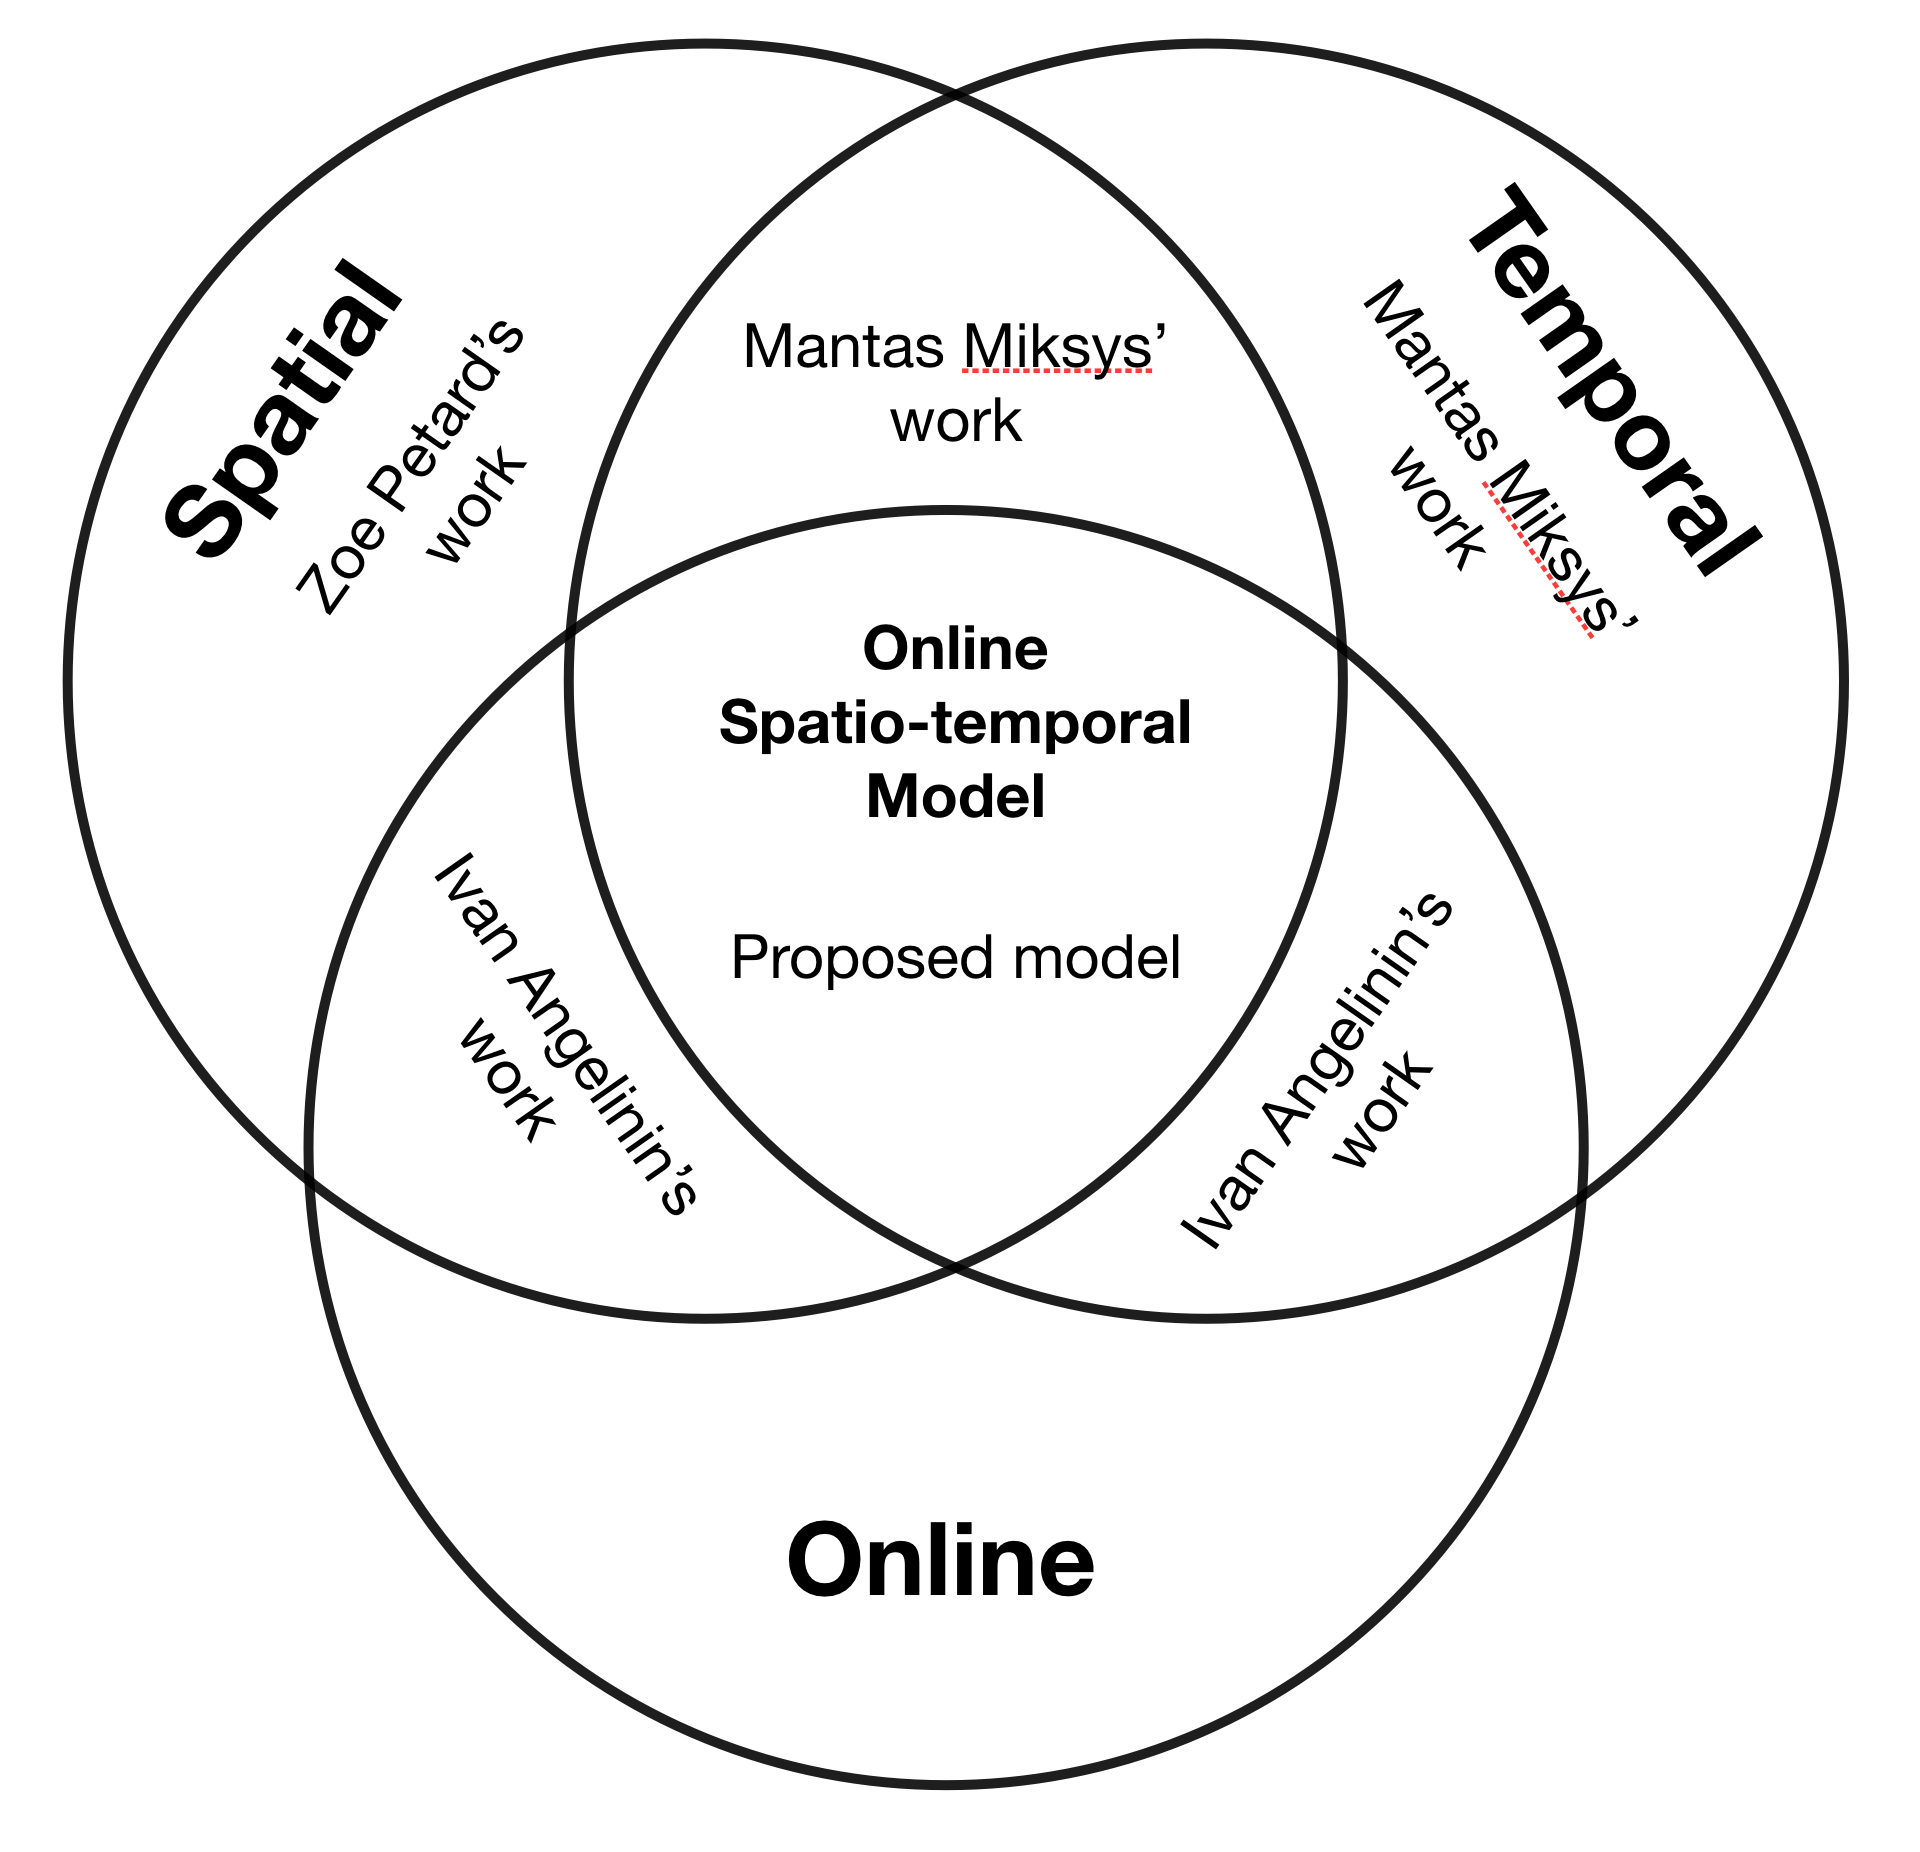
\includegraphics[width=.6\textwidth]{images/venn_diagram.png}
    \caption{Comparison of previous models}
    \label{fig:venn_diagram}
\end{figure}

%\subsection {Predicting Air Quality using Personal Exposure Monitors on Cyclists}
%This project was done by Aart Meijer in \hl{} and used 

\subsection {Predictions of PM2.5 and PM10 Concentrations Using Static and Mobile Sensors}

Mantas Miksys' 2016  project \cite{mantas} involved implementing and comparing offline temporal models and online spatial models using only static sensors for training and mobile sensors for validation. He also presented an offline spatio-temporal prediction model using only stationary sensors.  The models tested included Artificial Neural Networks, Decision Trees and others for temporal predictions and Inverse Distance Weighting, Kriging and Radial Basis Functions for spatial predictions. His work helped to define baselines and evaluation metrics for the model, and understand the temporal and spatial components of predictions.
The work presented differs in the way that this one is online, possible to implement for real-time application and can use mobile sensors' data collected in different time periods and different locations simultaneously with static sensor's data.

\subsection {Sensing Spaces: Improving Spatial and Temporal Prediction of Air Pollution Using Online Learning Algorithms}

Ivan Angelinin's 2018 project \cite{ivan} compared several approaches of online temporal models and online spatial models. He tested the following temporal models: Multilayer Perceptron, Linear Regression with Stochastic Gradient Descent, and Passive-Aggressive Regressor, and the following spatial models: Kriging and Radial Basis Functions. Although Angelinin's analysis of temporal and spatial models did not have any connection between themselves, it was instrumental in understanding how models performed and helped to choose models to use for the spatio-temporal model. Angelinin's code from the temporal and spatial model was not used, and code for this project was implemented from scratch using the same helper libraries that Ivan used in his work.


\subsection{Sensing Spaces: Planning journeys with least polluted, shortest routes in urban environments}
The work by Stefan Ivanov in 2018 \cite{stefan} consisted of making an application that performed route planning to find the least polluted route between a source and a destination on a map. This is an example of a potential application for the model presented in this report.

\subsection{Personal Exposure to Air Pollution with Different Modes of Transport and Urban Environments Using Wearable Sensors}

This project had a different scope. Mihai Visuian, in 2018, used mobile sensor data to classify urban environments and modes of transport using both supervised and unsupervised models\cite{mihai}.

\subsection{High Resolution Spatial Predictions of Air Pollution Levels in Edinburgh}
Zoë Petard \cite{zoe} developed the most recent work on the Sensing Spaces project. She implemented a convolutional neural network for spatial predictions of PM values using stationary data and validated on mobile data. She also collected data from stationary and mobile sensors throughout the project. Although this project is very different from what is proposed, her work was useful as the dataset and calibration factors were taken from this project for the model prediction experiments in this report.
\cite{zoe}




\section{Related Work}

\subsection{Online spatio-temporal models}

During the literature survey, no papers of an online spatio-temporal model for predicting air pollution levels were found. However, several applications of online spatio-temporal models were found for the most diverse applications: Hwa-Lung Yu \textit{et al.} produced an online spatio-temporal model to apply in epidemic dispersion of dengue fever in Taiwan. \cite{epidemic}, Gurkirt Singh \textit{et al.} applied and presented a solution for video frame prediction and action localisation. They stated in 2014 that in their field of study "current state-of-the-art approaches work offline, and are too slow to be useful in real-world settings" \cite{frame_pred}, , and for that reason, they published a paper that would allow for real-world settings. Lastly, a PhD thesis by Harold Soon Hong Soh entitled "Online spatio-temporal learning and prediction for adaptive robotic systems" \cite{robotics} focused on the robotics field, particularly tactile classification and learning assistance.

\subsection{Particulate matter concentration predictions}

Regarding air pollution predictions, the current state of the art is aligned with previous work performed in the Sensing Spaces project. Comparable work performed in Zurich \cite{zurich} shows an improvement in spatio-temporal models with a spatial resolution of $100 m \times 100 m$ and semi-daily temporal resolution using land-use and traffic characteristics. Both the work of Hasenfratz \textit{et al.} and this report aim at improving "detailed real-time pollution assessment" \cite{zurich}, and both used mobile data to make predictions: in Hasenfratz \textit{et al.} case with sensors installed in public buses. Their challenges such as "very sparse ground truth data", was a common problem in this project.

Huiping Peng's thesis \cite{peng} implemented, compared and evaluated the application of machine learning methods to air quality prediction using six stationary sensors in six different Canadian cities. Interestingly, this work included an online machine learning method entitled "Online Sequential Multiple Linear Regression" but the concept of using mobile sensors as additional data was not studied and predictions had a daily temporal scale of 24 hours.

Schneider \cite{low_cost} describes the use of low-cost sensors, a model that describes patterns of urban air pollution and data fusion techniques to make hourly predictions of nitrogen dioxide concentration in simulated data and real data in Oslo, Norway.

Another branch of machine learning, deep learning has been applied to air quality interpolation, prediction and feature analysis \cite{qi}. However, no reference of online learning or real-time application of deep learning was found in Qi's work of 2018. Spatio-temporal deep learning is also applied in the literature in other contexts such as traffic flow and high-frequency trading \cite{trading}.


Lastly, there are several model-based approaches to modelling pollution particles dispersion such as ADMS and AERMOD, developed in the United Kingdom, The Numerical Atmospheric-dispersion Modelling Environment (NAME), developed and used by the Met Office, RIMPUFF, a dispersion modelling system developed in Denmark, and CALPUFF, a meteorological and air quality modelling system produced in the United States of America. These are models that predict the dispersion of air pollutants, meteorological and air quality events in long-range events, especially compared to the PM predictions in this project.

\chapter{Improved user interface for AIRSpeck mobile app}

The Public Health Initiative on Low- and Middle-Income Countries Air Pollution (PHILAP) is a study funded by the Medical Research Council that aims to study the health effects of air pollution in Delhi, India and other low- and middle-income countries, with a multidisciplinary team, including Data scientists and Social scientists. It will use RESpeck and Airspeck sensors to measure personal exposure to air pollution together with the stationary AIRSpeck while simultaneously measuring respiratory rate/flow and activity levels (with the RESpeck), to correlate this data with progress of respiratory diseases. This quantitative information will be allied with qualitative data such as the socio-geographic and cultural context of people's lives through the Social Sciences dimension of the study, for example with interviews with the participants, aiming to foster the dialogue between multiple disciplines to develop shared ways of analysing different types of datasets of air pollution.

The PHILAP pilot study, intended to reproduce in a smaller scale the deployment of these sensors and data collection techniques, as a trial for the bigger scale study in Delhi, India, where other studies are occurring with the same set of sensors, such as the Delhi Air Pollution: Health and Effects (DAPHNE) study. It also aims to engage with methodologies and challenges of working across distinct research methodologies.

The objective of this part of the project was to implement the requirements for the study from a technological point of view, recruit, organise and put into practice the data collection with participants. The task included the process of ethics approval by the School of Informatics following the data protection training course.

It is hoped that this data from the PHILAP study together with the online learning methods developed in this project will be employed in Part II of the Minf dissertation.

\section{Principles}

An application was developed by the Centre for Speckled Computing of The University of Edinburgh \cite{air-respeckapp} that connects to the sensors and records the values read into the smartphone's storage. However, that application did not include the capability of recording qualitative data such as photos, video, sound, and text. Those features were developed and integrated into the application that already existed. In addition, the User Interface was improved to allow easier access to the new features. The functional requirements for the features were:

\begin{itemize}
\item The user should be able to take a photograph, visualise and choose to save or discard that photograph.
\item The user should be able to record a video, visualise and choose to save or discard that video.
\item The user should be able to record an audio clip, reproduce it and choose to save or discard that clip.
\item The user should be able to save a text comment and save it.
\item All photographs, videos, audio recordings, and text comments should be time stamped for further analysis and synchronisation with other data (i.e., quantitative data).
\item The media collected should be saved in a folder inside the data collection folder to facilitate its upload to the servers along with the quantitative data collected.
\item The user should easily identify and select the data that they need to collect.

\end{itemize}

The following general principles of User Interface Design \cite{ui_design} were followed during implementation:

\begin{itemize}
    \item \textbf{Consistency, Aesthetically Pleasing, Predictability and Grouping:} The buttons created are consistent with the other buttons and grouped in their own section of the screen, indicating interactivity to the user. The format is familiar to the rest of the interface.
    \item \textbf{Directness, Clarity and Simplicity:} The user can access the function easily and complete a media collection cycle in three button presses: select type, capture and accept capture (except audio recording which requires four button presses). Buttons also become inactive if the action cannot be made at that moment.
    \item \textbf{Forgiveness, Control and Recovery:} The user has the control to review and accept or reject the media captured and is allowed to return to the main screen easily at any point of the media collection cycle.
\end{itemize}

\section{Implementation}

Figure \ref{fig:prototypes}, presents some prototypes designed to simulate the feature and facilitate discussion about the best way to implement this feature. As an output of the debate, given that the application is used in several countries such as the United Kingdom and India, with several different languages, it was opted to use icons instead of text to make the feature universally intuitive and usable (see Figure \ref{fig:main}). It was also essential to make the feature easily accessible, to decrease the difficulty for the users to collect data; therefore, the functionality was integrated into the subject mode screen of the application.

The features were developed in Android Studio using the Java programming language. The icons used were taken from Font Awesome, under CC BY 4.0 licence \cite{fontawesome}. 

\begin{figure}[H]
\begin{center}$
\begin{array}{lll}
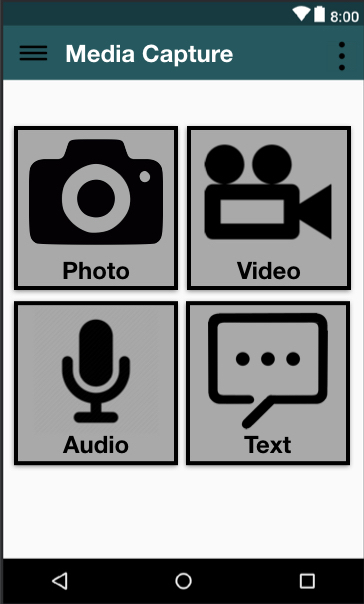
\includegraphics[width=.3\linewidth]{images/prototypes_001}&
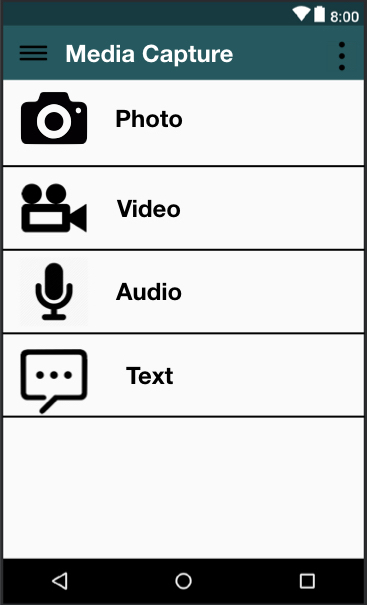
\includegraphics[width=.3\linewidth]{images/prototypes_002}&
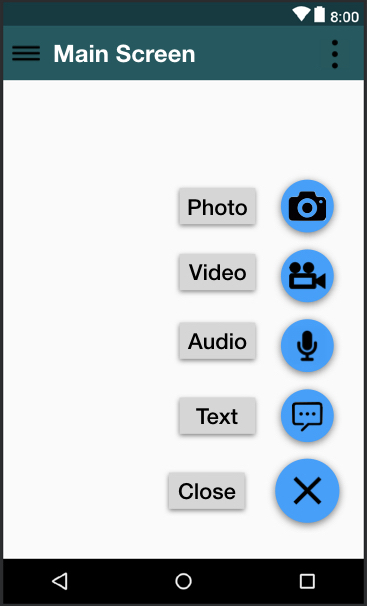
\includegraphics[width=.3\linewidth]{images/prototypes_003}
\end{array}$
\end{center}

\begin{center}$
\begin{array}{rr}
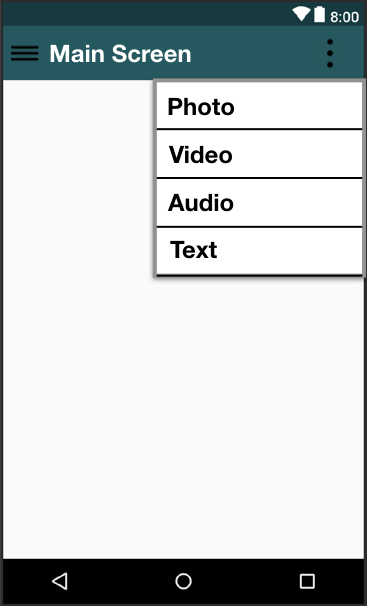
\includegraphics[width=.3\linewidth]{images/prototypes_004}&
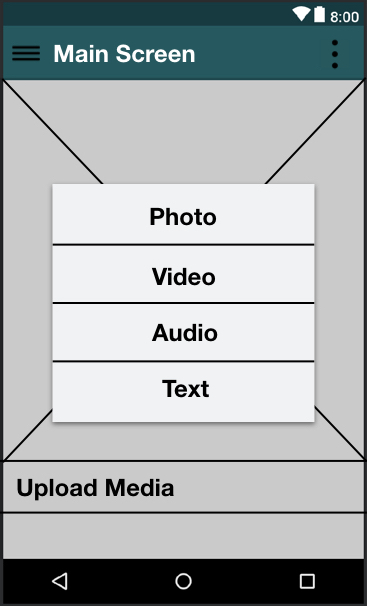
\includegraphics[width=.3\linewidth]{images/prototypes_005}
\end{array}$
\end{center}
\caption{Mock-ups of the feature}
\label{fig:prototypes}
\vspace{1cm}
\end{figure}


The final implementation included four buttons and their respective behaviour flow and is shown in Figure \ref{fig:main}. Each of the buttons intuitively indicates and launches a subsection of the feature: either the camera for photos and video recordings, the audio screen, shown in Figure \ref{fig:extras}, or the text comment dialog also shown in the same figure.

\begin{figure}[H] 
 
  \begin{minipage}[b]{0.5\linewidth}
    \centering
    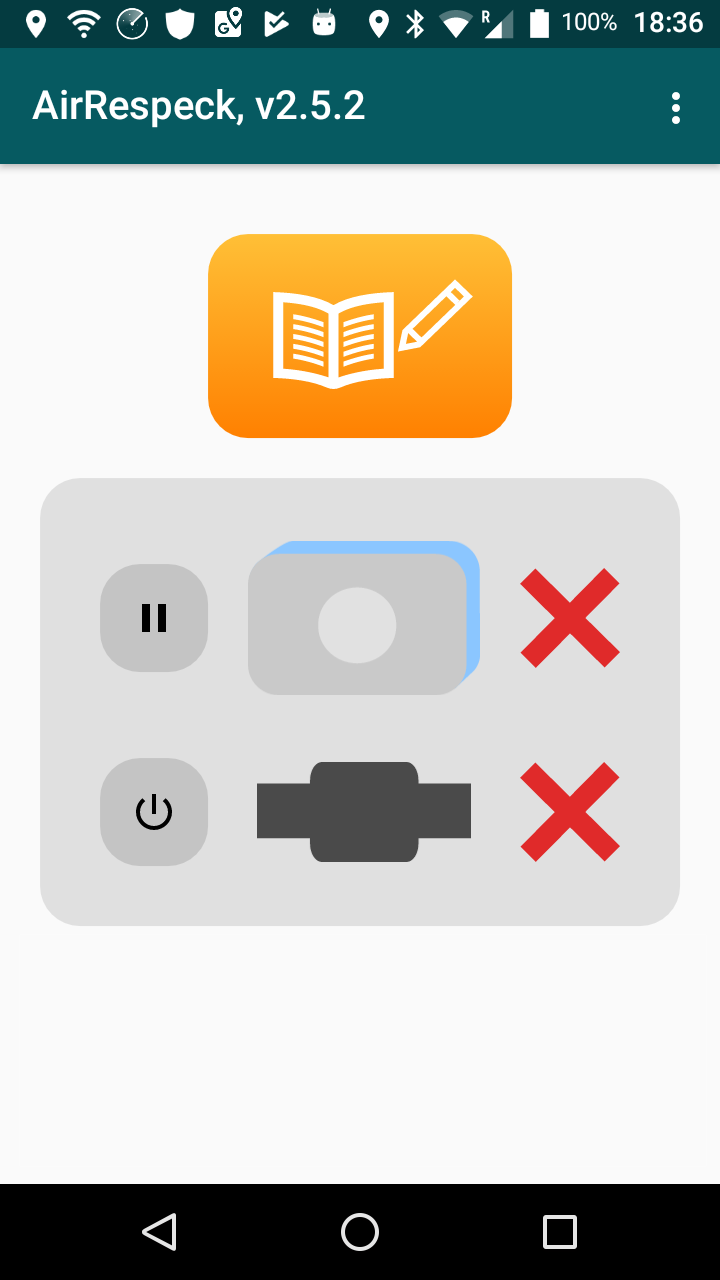
\includegraphics[width=.8\linewidth]{images/main_before} 
    \vspace{3ex}
  \end{minipage}%% 
  \begin{minipage}[b]{0.5\linewidth}
    \centering
    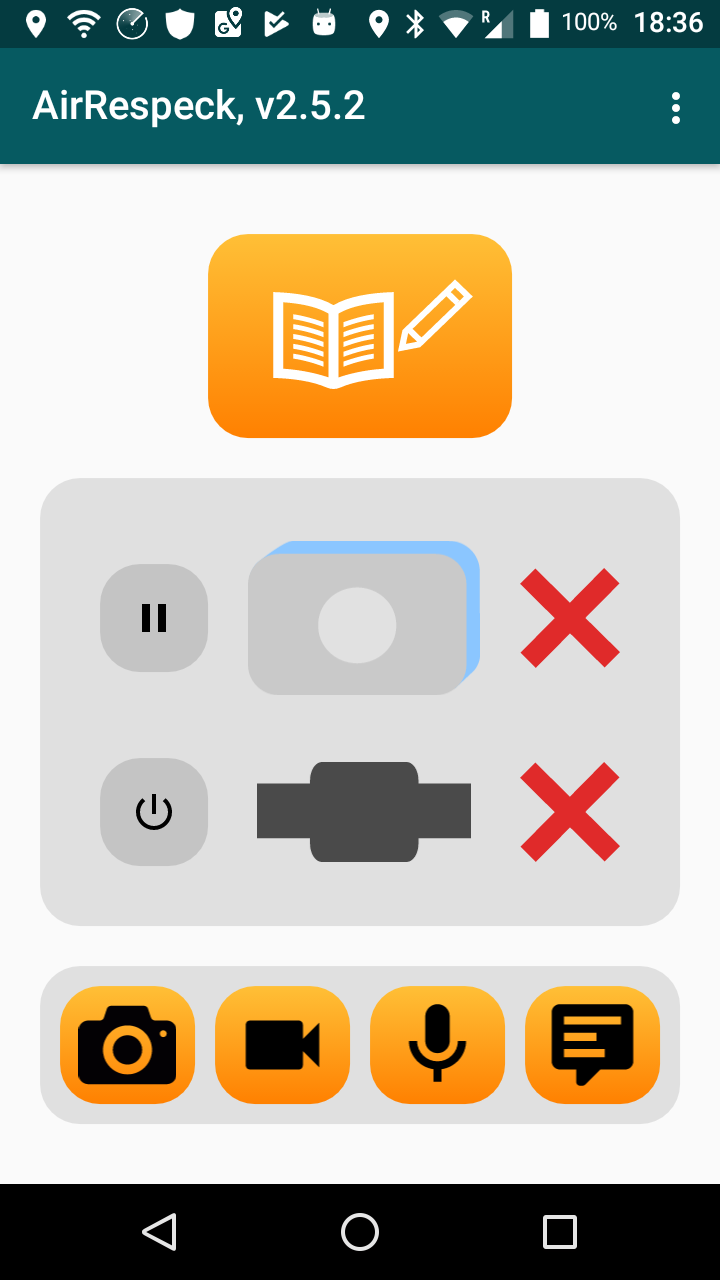
\includegraphics[width=.8\linewidth]{images/main} 
    \vspace{3ex}
  \end{minipage} 
  \caption{Subject mode before (left) and after (right) implementation }
  \label{fig:main}
  \vspace{0.5cm}
  \begin{minipage}[b]{0.33\linewidth}
    \centering
    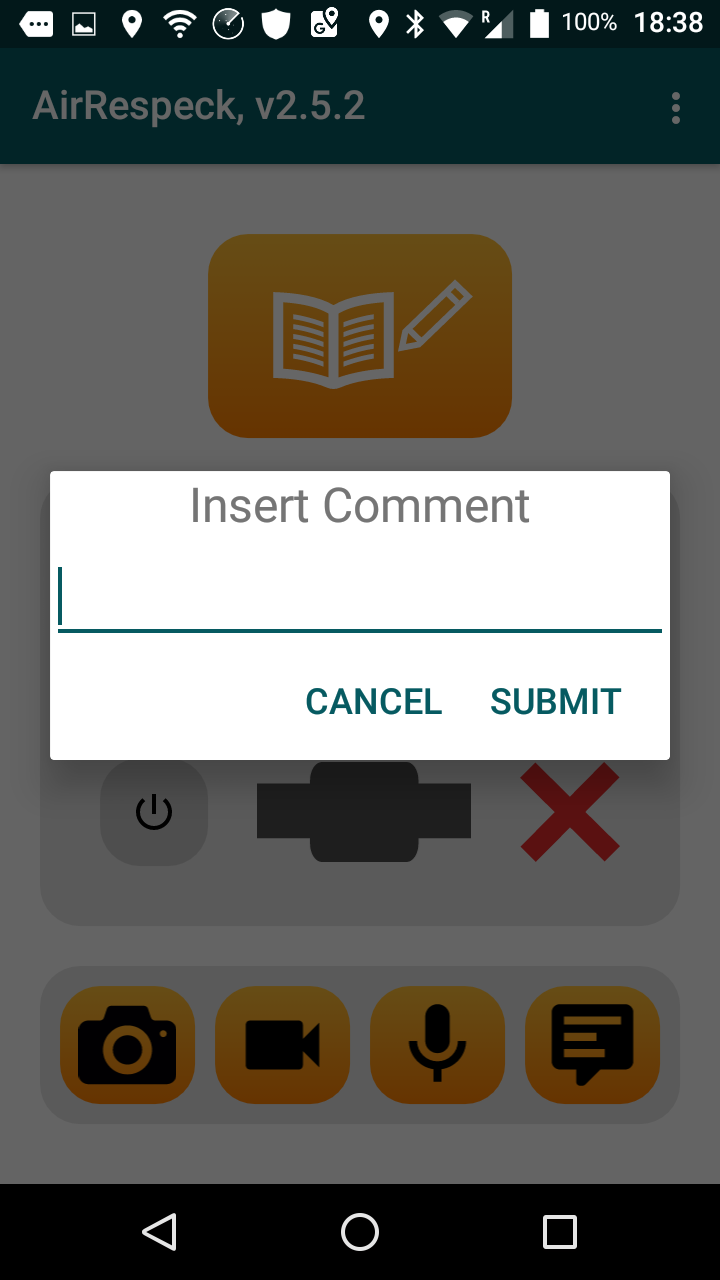
\includegraphics[width=.8\linewidth]{images/text} 
    \vspace{3ex}
  \end{minipage}%%
  \begin{minipage}[b]{0.33\linewidth}
    \centering
    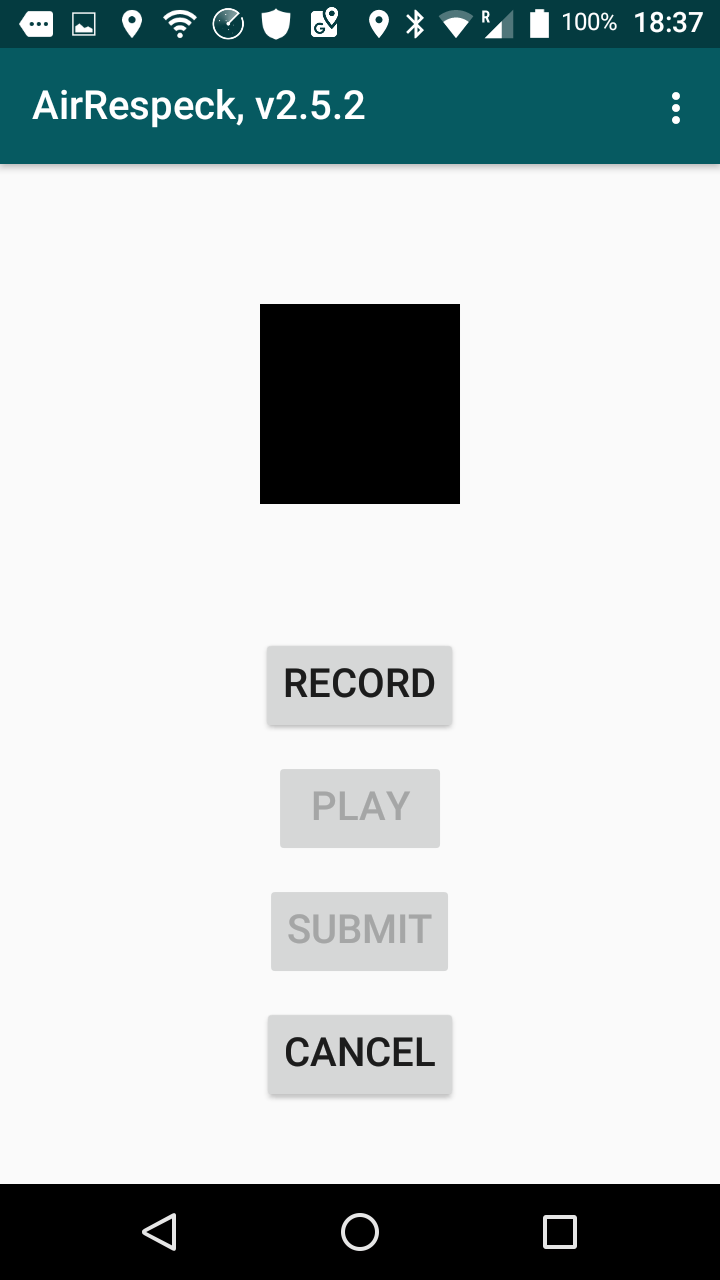
\includegraphics[width=.8\linewidth]{images/audio} 
    \vspace{3ex}
  \end{minipage}%%
  \begin{minipage}[b]{0.33\linewidth}
    \centering
    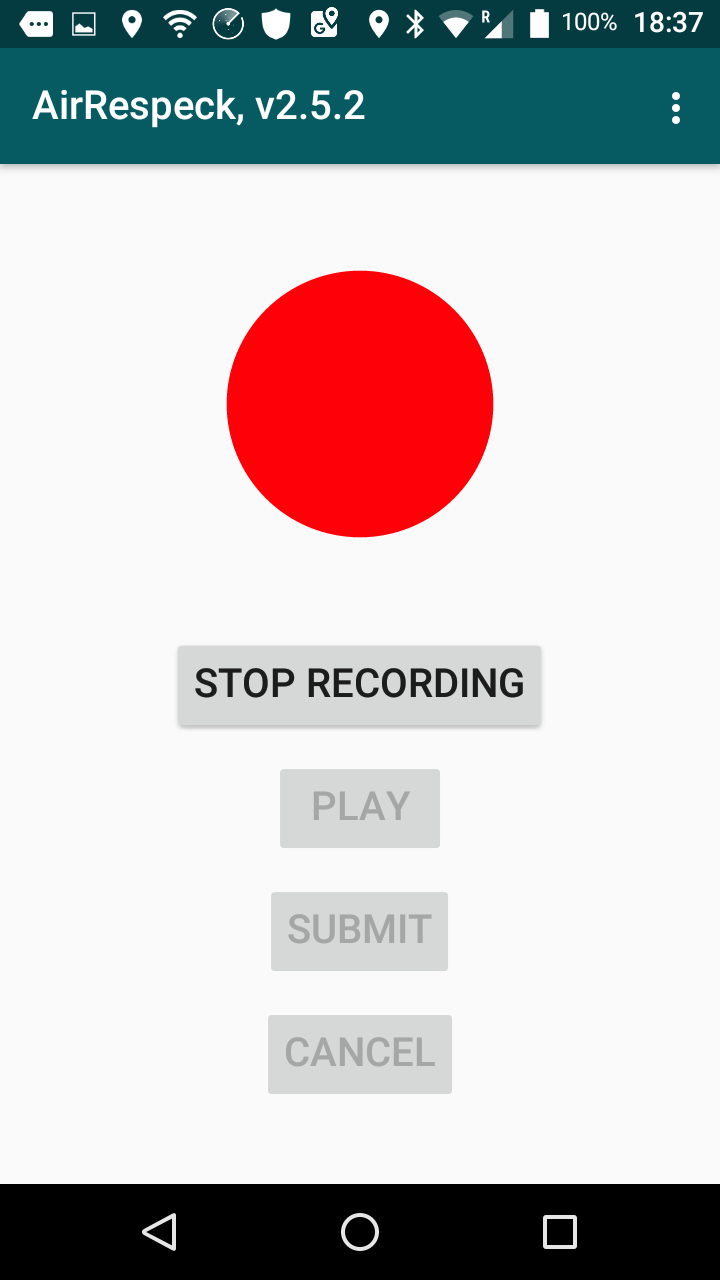
\includegraphics[width=.8\linewidth]{images/recording} 
    \vspace{3ex}
  \end{minipage} 
  \caption{Comment dialog (left), Audio Clip screen stopped (centre) and recording (right)}
  \label{fig:extras}

\end{figure}


\subsection{Data collection}
In order to be allowed to collect data from participants, an \textit{Information Sheet} was produced to provide to the participants in the pilot study. This document included all the details about the study and can be found in Appendix \ref{sec:infosheet}. The participants signed the School of Informatics' template for participation consent, presented in Appendix \ref{sec:consent}. 
To apply for ethics approval from the School of Informatics, the author studied an online data protection training course provided by the university and, in conjunction with the documents described above, obtained the approval to collect the data.
Students were asked to wear one AIRSpeck-P and a RESpeck sensor to collect breathing data and particulate matter in the environment. The RESpeck device was worn below the left rib, and the AIRSpeck was worn externally, like a belt. Students were provided with a phone connected to the sensors and were asked to observe and log information about air pollution and breathing sensations in the form of text, audio, photos or video clips, using the feature recently implemented.

\section{Results and analysis}

\subsection{Data visualisation}
A Python script was produced using Pandas \cite{pandas}, Matplotlib \cite{matplotlib}, Numpy \cite{numpy} and gmplot \cite{gmplot} to plot the air pollution and media collected data on a map and allowed to visualise the air pollution data collected with the participants and to incorporate the type of media used for collectioncollected into such visualisation. This program outputs, for every participant, an HTML file that lays on top of a map from Google Maps \cite{googlemapsapi}, circles with the air pollution readings coloured according to the value read and black markers that indicate the location of the media collected by the user. Hovering with the mouse on the black markers show the corresponding name of the file where such data was stored, allowing to connect the qualitative data to the quantitative data showed on the map. The fact that it is an HTML file with a Google Maps layer allows for the visualisation to be interactive with zoom and pan features. In addition, the program outputs an image with the legend of the circles' colours. An example of both outputs can be seen in Figures \ref{fig:map} and \ref{fig:scale} below.


\begin{figure}[H] 
\centering
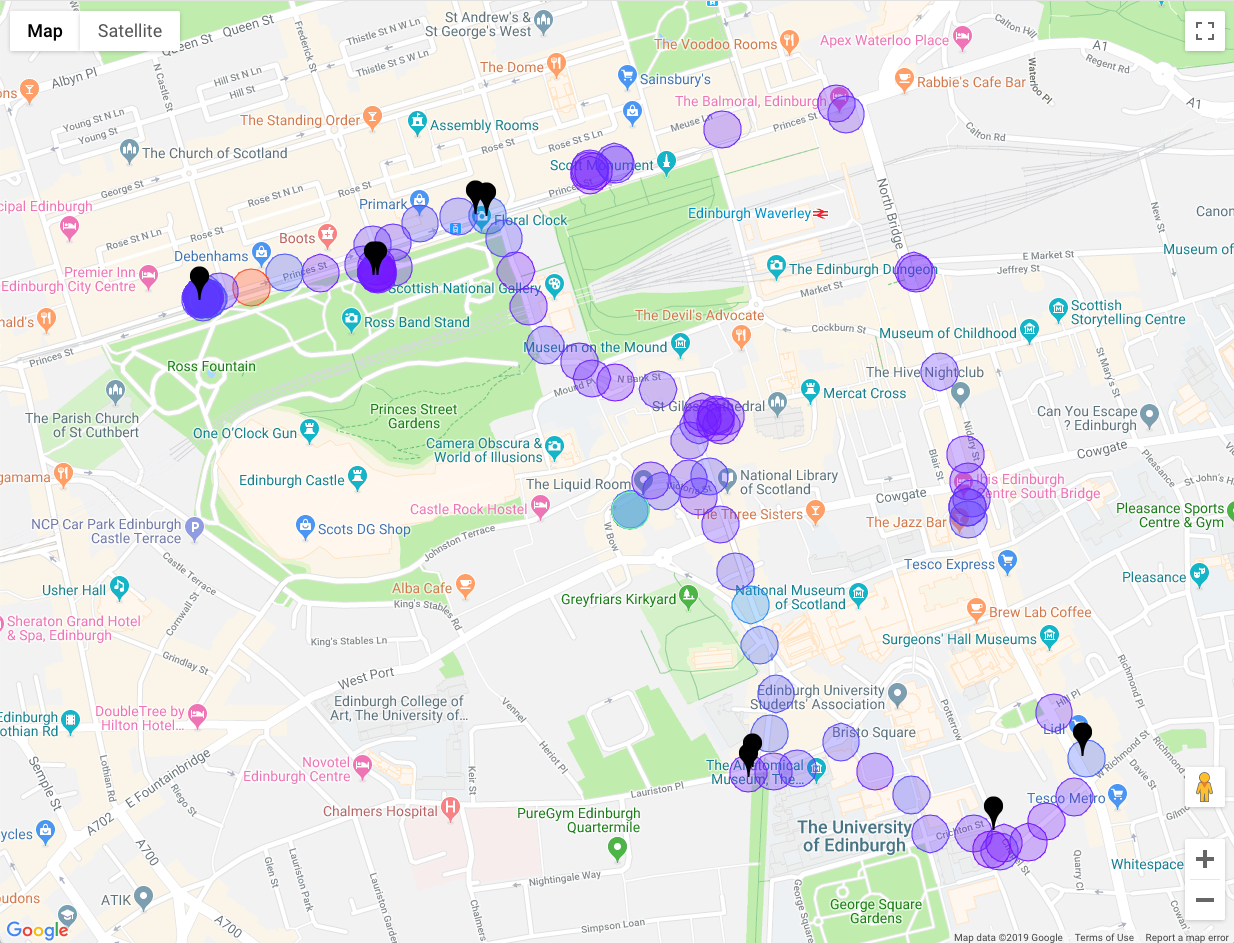
\includegraphics[width=\linewidth]{images/map_PHP001} 
\caption{Map and PM2.5 readings of Participant \#1}
\label{fig:map}
\vspace{0.5cm}
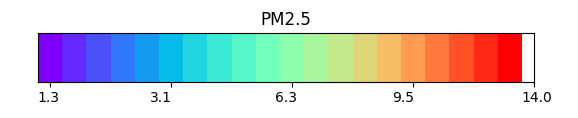
\includegraphics[width=.8\linewidth]{images/legend_PHP001} 
\caption{Legend corresponding to Participant \#1 PM2.5 data} 
\label{fig:scale}
\end{figure}


In the pilot study, ten people participated and collected data from two trips they performed in their daily routine: from home to work or university and vice-versa. During this period, they were asked to wear the AIRSpeck and RESpeck sensors and to use the media collection feature on the smartphone provided as they saw fit. Data collection took place between 10th October and 15th November 2018. Participant \#6 did not collect data correctly due to their misuse of the equipment.


Out of the 10 participants, 7 utilised the new media collection feature at least once. The feature was used a total of 41 times and Figure \ref{fig:mediacollected} shows a breakdown of the utilisation of the feature by media type. The most commonly used type of media collected and usually preferred was photos, followed by a similar number of text comments and video clips and lastly the least preferred option was audio clips which were used only three times.

\begin{figure}[H]
    \centering
    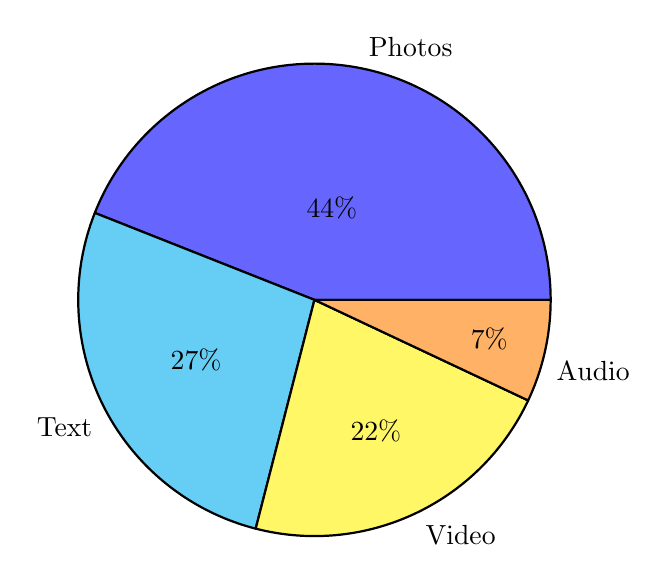
\begin{tikzpicture}
    \pie{44/Photos, 27/Text, 22/Video, 7/Audio}
    \end{tikzpicture}
    \caption{Breakdown of media collection by type}
    \label{fig:mediacollected}
\end{figure}

Each participant had different exposures to air pollution data. Some statistics were computed individually for each participant, presented below in Table \ref{tab:philapstats}. This information helps to interpret personal exposure of particulate matter. 

\begin{table}[H]
\centering
\resizebox{\textwidth}{!}{%
\begin{tabular}{l|cccc}
 & \textbf{\begin{tabular}[c]{@{}c@{}}Average PM1 \\ exposure\end{tabular}} & \textbf{\begin{tabular}[c]{@{}c@{}}Average PM2.5 \\ exposure\end{tabular}} & \textbf{\begin{tabular}[c]{@{}c@{}}Average PM10 \\ exposure\end{tabular}} & \textbf{\begin{tabular}[c]{@{}c@{}}Maximum PM2.5 \\ value read\end{tabular}} \\ \hline
\textbf{Participant 1} & 1.70 & 2.38 & 6.67 & 14.01 \\
\textbf{Participant 2} & 1.31 & 2.35 & 13.51 & 18.50 \\
\textbf{Participant 3} & 1.42 & 2.10 & 8.16 & 4.49 \\
\textbf{Participant 4} & 0.66 & 1.03 & 4.03 & 4.72 \\
\textbf{Participant 5} & 0.72 & 1.01 & 3.28 & 2.27 \\
\textbf{Participant 7} & 8.24 & 10.37 & 20.64 & 26.26 \\
\textbf{Participant 8} & 0.71 & 1.26 & 27.38 & 4.54 \\
\textbf{Participant 9} & 1.54 & 2.61 & 18.61 & 16.47 \\
\textbf{Participant 10} & 1.88 & 2.85 & 25.40 & 34.22
\end{tabular}%
}
\caption{Participants' statistics}
\label{tab:philapstats}
\end{table}

Interestingly, Participant \#7 measured unusually high values of PM2.5 exposure compared to other participants. The path that the participant took while collecting data can justify the high exposure values as the majority of the route was along a big construction site where a shopping centre was, being demolished and redeveloped, at the east end of Princes Street.

It is planned that in Part II of this project, data coming from the PHILAP project will be analysed in detail and converge with the online spatio-temporal models described in this project.

\chapter{Methodology: Online Spatio-temporal Model}
The objective of this part of the project was to create an online spatio-temporal machine learning model that could predict, using static sensors (AIRSpeck-S) and mobile sensors (AIRSpeck-P) data, the concentration levels of particulate matter in the near future (up to 6 hours). This model needs to be able to make predictions in space and time and adapt continuously in an online setting, with the expectation of being used in a real-time scenario. This model could have multiple applications such as warning system for vulnerable people, route planning, pollution monitoring and facilitate political and environmental decision making.

This project focused on making predictions of PM2.5 values given its far-reaching impact on the community and individual health conditions; however, the work described below can be applied to other PM values as well.


\section{Dataset}

The experiments performed use data that was collected by Zo\"e Petard (ZP) between June 3rd 2018 and June 26th 2018 \cite{zoe}. To simulate a real-time application of the model, two specific time periods within this dataset were chosen, given their continuity of stationary sensor readings. The first one between 3rd June 2018 to 6th June 2018, referred to as dataset A, and the second one from 23rd June 2018 to the 26th June 2018, referred to as dataset B. The datasets include continuous data from six stationary sensors and one period of mobile data collection per day, averaging $53$ minutes of mobile data per day. 

The test area is a region defined by a quadrilateral of size $0.97km$ (latitude) and $0.96km$ (longitude) in the central area of Edinburgh, totalling an area of $0.93 km^2$. This region was subdivided into a $20 \times 20$ grid, forming 400 cells of approximately $48m \times 48m$ each in size. All data was converted to these grid cells location using a Cartesian coordinate system as seen in Figure \ref{fig:grid}, using the grid cell as the resolution of the model. This level of resolution is greater than any work before ZP's spatial model \cite{zoe}.
In Figure \ref{fig:grid}, it is also possible to see the location of the stationary sensors, described in more detail in Table \ref{tab:sensors}. This table also includes information about the two mobile sensors used to collect data over several cell grids. This data is sparse both temporally, because of the duration of the collection periods and spatially, because at most one cell grid was being measured by mobile sensors at any point in time. This presented challenges to include this data in the training phase of the model created.


\begin{figure}[h] 
\centering
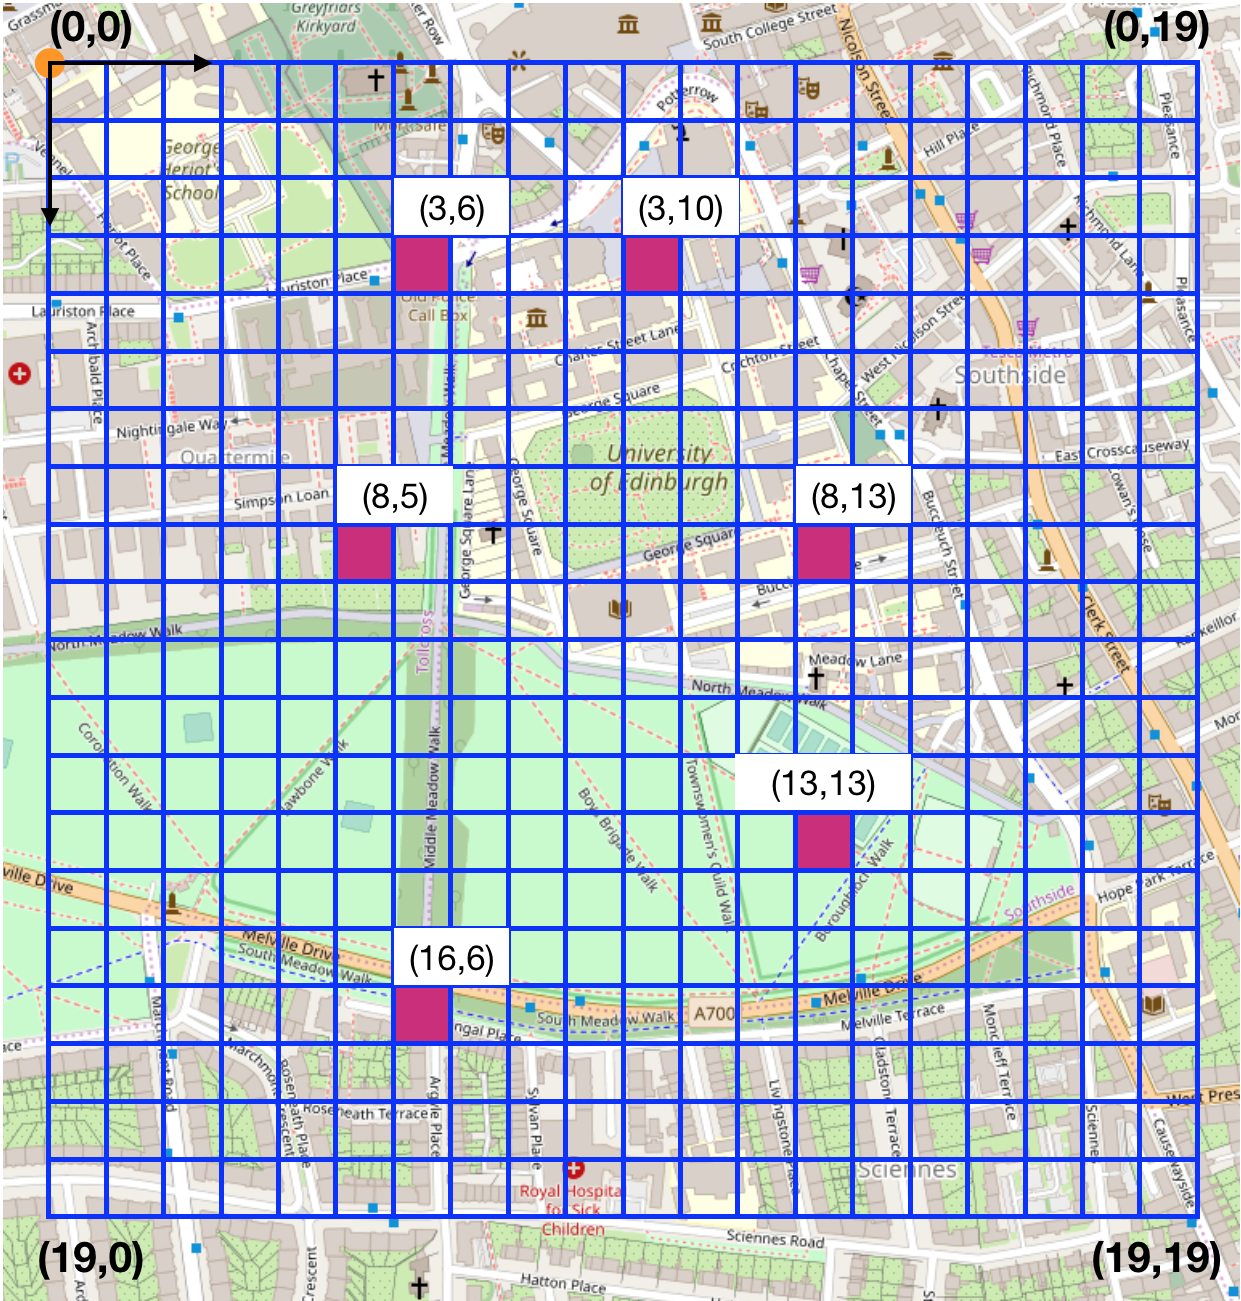
\includegraphics[width=0.8\linewidth]{images/mapa_com_pontos} 
\caption{Map of the test area and grid overlay. Purple cell grids indicate the locations of the stationary sensors. The coordinate system origin is marked in orange. }
\label{fig:grid}
\end{figure}

\begin{table}[h]
\centering
\resizebox{\textwidth}{!}{%
\begin{tabular}{c|ccc|ccc}
\textbf{Sensor Name} & \textbf{Sensor Identifier} & \textbf{Grid Row} & \textbf{Grid Column} & \multicolumn{3}{c}{\textbf{Calibration Factors}} \\ \cline{5-7} 
 &  &  &  & PM2.5 & Temperature & Humidity \\ \hline
Melville (MV) & 02E5F77764B873DA & 16 & 6 & 1.0 & 1.0 & 1.0 \\
Lauriston (LT) & E5FD8C55EAA37555 & 3 & 6 & 1.22 & 1.19 & 1.01 \\
Library (LY) & 200A7CED9D597407 & 8 & 5 & 1.55 & 1.51 & 1.00 \\
Tennis Court (TC) & AA0E63CF5118F98F & 13 & 13 & 2.38 & 2.31 & 0.98 \\
Bristo Square (BS) & B61241EF668DBC2C & 3 & 10 & 2.34 & 2.22 & 0.98 \\
Buccleuch Place (BP) & E786F1568F65C296 & 8 & 13 & 7.08 & 7.05 & 0.97 \\
Mobile 1 & XXM007 & - & - & 4.86 & 1.16 & 0.74 \\
Mobile 2 & XXM008 & - & - & 4.91 & 1.19 & 0.74
\end{tabular}%
}
\caption{Description of sensors and calibration factors used, with Melville sensor as reference.}
\label{tab:sensors}
\end{table}

The static sensors collected data over both datasets every 5 minutes, however, the temporal window used was 15-minute windows. This choice is justified for being not too big to allow mobile data integration, which was sampled every 10 seconds, and not too small to discern noise in the data readings. The readings were therefore re-sampled to 15 minutes using the arithmetic mean to group these values.


Figures \ref{fig:2d_mobile} and \ref{fig:hist_mobile} show the sparsity of mobile data over the grid in both datasets A and B. Almost all cell grids include less than ten readings and $45\%$ of the cells were not visited by the mobile sensor during data collection. It is possible to observe one particular grid cell with more mobile data readings because that cell is the usual location where people collecting data would start and stop using the sensor, corresponding to the Informatics Forum building. 

\begin{figure}
\centering
\begin{minipage}{.5\textwidth}
  \centering
  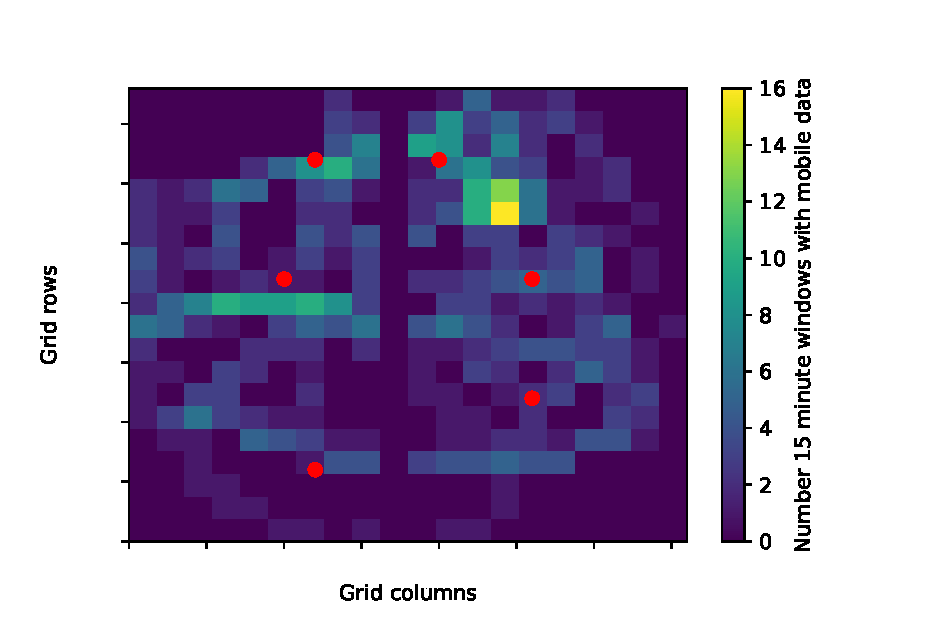
\includegraphics[width=\linewidth]{images/2D_mobile_data.eps}
  \captionsetup{width=.9\linewidth}
  \captionof{figure}{2D visualization of mobile data collected in both datasets}
  \label{fig:2d_mobile}
\end{minipage}%
\begin{minipage}{.5\textwidth}
  \centering
  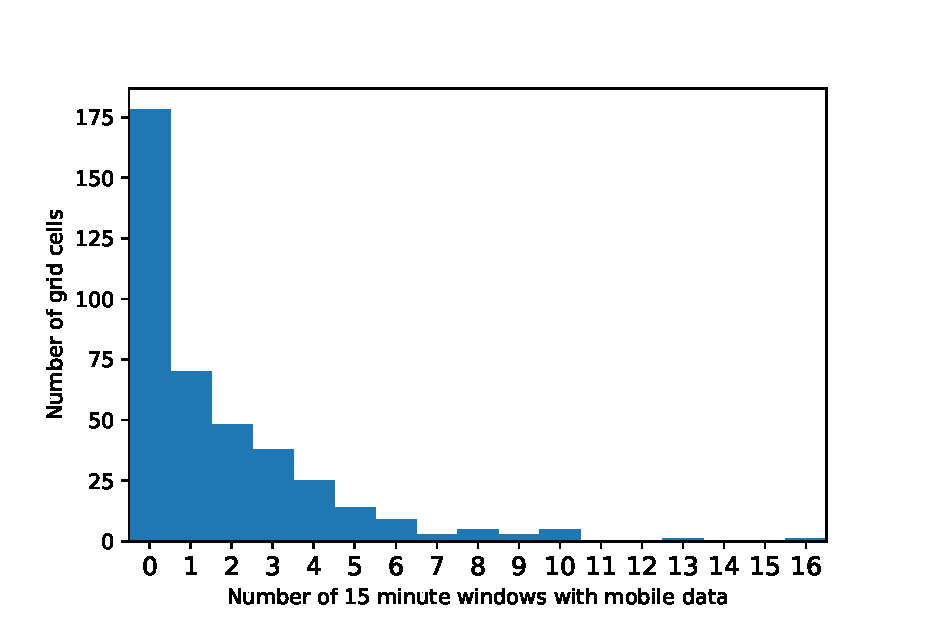
\includegraphics[width=\linewidth]{images/histogram_mobile.eps}
  \captionsetup{width=.9\linewidth}
  \captionof{figure}{Histogram of grid cells by amount of mobile data collected in both datasets}
  \label{fig:hist_mobile}
\end{minipage}
\end{figure}



\subsection{Data calibration}

Similar to ZP's work, the readings of the different sensors were calibrated in reference to one of the sensors. ZP co-located the sensors in the laboratory and used the data collected during that time to calculate the factors needed for a linear scaling, presented in Table \ref{tab:sensors}. I used these factors to calibrate both stationary and mobile sensor data in both datasets.

\subsection{Outlier removal}
As another pre-processing step, outlier detection was performed on the stationary sensor data of dataset A by visual inspection (see Figure \ref{fig:raw_with_outliers}). The outliers were removed and substituted by the average of its corresponding previous and next value. Three outliers were removed by this process, and the dataset after removal can be seen in Figure \ref{fig:raw_without_outliers}. Outliers were not removed in dataset B to be able to measure the performance of the model without outlier removal, to be able to emulate a real-time use case where data was not pre-processed (other than calibration).

\begin{figure}[H] 
\centering
\vspace{1cm}
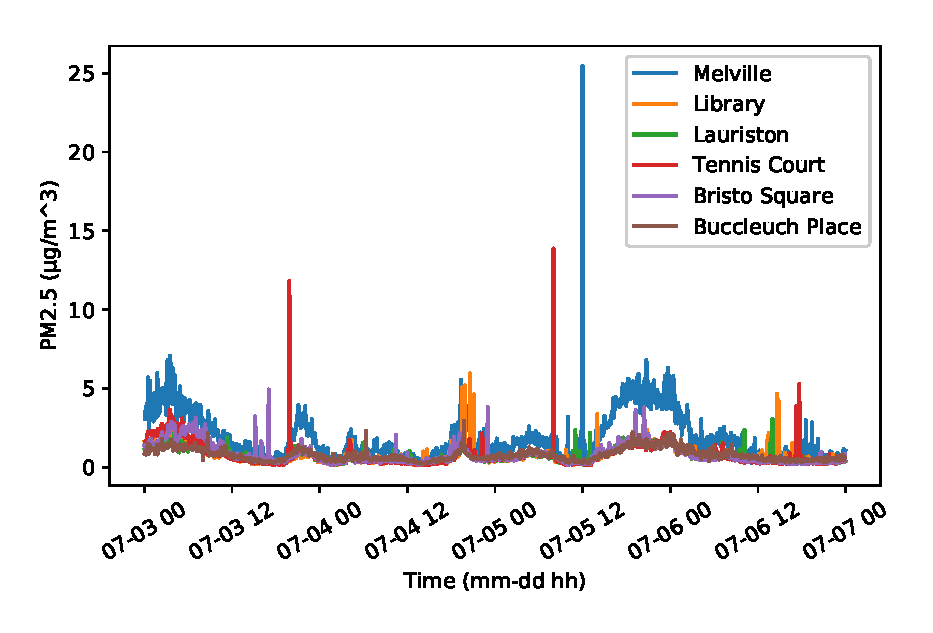
\includegraphics[width=\linewidth]{images/calibrated_data.eps} 
\caption{Calibrated readings of stationary sensors on dataset A with outliers.}
\label{fig:raw_with_outliers}
\vspace{1cm}

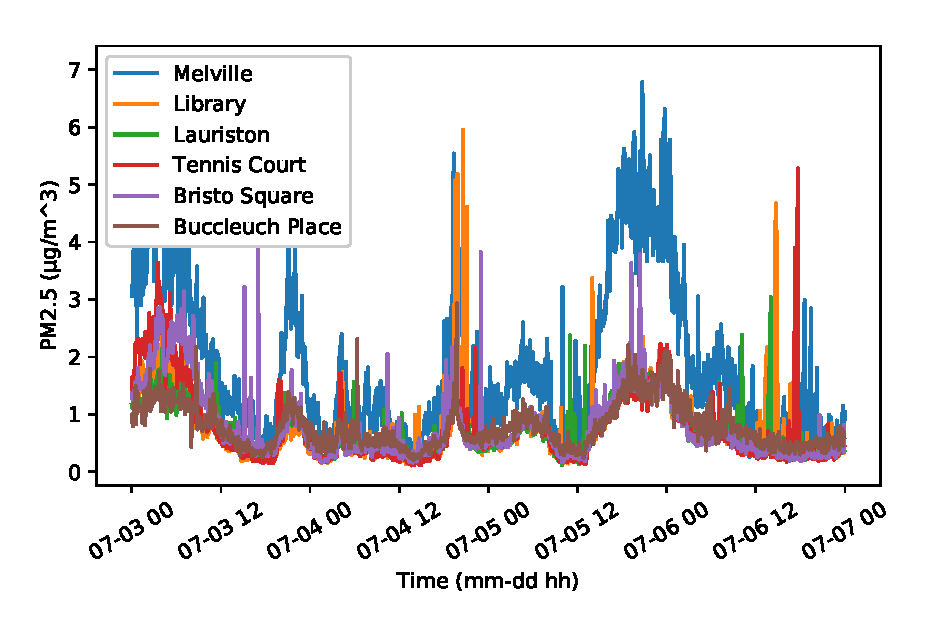
\includegraphics[width=\linewidth]{images/calibrated_data_no_outliers.eps} 
\caption{Calibrated readings of stationary sensors on dataset A without outliers.}
\label{fig:raw_without_outliers}
\vspace{1cm}

\end{figure}


\begin{table}[h]
\centering
\resizebox{\textwidth}{!}{%
\begin{tabular}{cc|cccccc|c}
\textbf{} & \textbf{Sensor} & MV & LT & LY & TC & BS & BP & \textbf{Overall} \\
\textbf{Statistical Property} & \textbf{} &  &  &  &  &  &  & \textbf{} \\ \hline
\multicolumn{2}{c|}{PM2.5 Average} & 1.83 & 0.73 & 0.75 & 0.74 & 0.80 & 0.77 & \textbf{0.94} \\
\multicolumn{2}{c|}{PM2.5 Standard Deviation} & 1.40 & 0.46 & 0.61 & 0.63 & 0.62 & 0.38 & \textbf{0.76} \\
\multicolumn{2}{c|}{PM2.5 Minimum} & 0.22 & 0.11 & 0.11 & 0.11 & 0.16 & 0.21 & \textbf{0.11} \\
\multicolumn{2}{c|}{PM2.5 Maximum} & 7.06 & 3.05 & 5.95 & 5.28 & 4.93 & 2.93 & \textbf{7.06} \\ \hline
\multicolumn{2}{c|}{Temperature average} & 18.89 & 12.28 & 9.21 & 6.6 & 6.95 & 2.43 & \textbf{9.39} \\
\multicolumn{2}{c|}{Temperature Standard Deviation} & 4.38 & 2.65 & 2.06 & 1.64 & 1.58 & 0.53 & \textbf{2.45} \\ \hline
\multicolumn{2}{c|}{Humidity Average} & 63.53 & 37.93 & 32.45 & 21.23 & 22.26 & 7.27 & \textbf{30.78} \\
\multicolumn{2}{c|}{Humidity Standard Deviation} & 13.98 & 8.14 & 6.61 & 5.18 & 4.99 & 1.54 & \textbf{7.74}
\end{tabular}%
}
\caption{Statistical properties of the calibrated static data of dataset A}
\label{tab:statisticsA}
\end{table}

\begin{table}[h]
\centering
\resizebox{\textwidth}{!}{%
\begin{tabular}{cc|cccccc|c}
\textbf{} & \textbf{Sensor} & MV & LT & LY & TC & BS & BP & \textbf{Overall} \\
\textbf{Statistical Property} & \textbf{} &  &  &  &  &  &  & \textbf{} \\ \hline
\multicolumn{2}{c|}{PM2.5 Average} & 1.09 & 0.44 & 0.45 & 0.50 & 0.51 & 0.53 & \textbf{0.59} \\
\multicolumn{2}{c|}{PM2.5 Standard Deviation} & 3.59 & 1.29 & 0.61 & 1.05 & 0.85 & 0.28 & \textbf{1.67} \\
\multicolumn{2}{c|}{PM2.5 Minimum} & 0.11 & 0.08 & 0.07 & 0.06 & 0.09 & 0.00 & \textbf{0.00} \\
\multicolumn{2}{c|}{PM2.5 Maximum} & 118.84 & 43.03 & 9.35 & 28.08 & 24.69 & 4.35 & \textbf{118.84} \\ \hline
\multicolumn{2}{c|}{Temperature average} & 21.36 & 13.68 & 10.08 & 7.02 & 7.66 & 2.55 & \textbf{10.38} \\
\multicolumn{2}{c|}{Temperature Standard Deviation} & 5.12 & 2.99 & 2.18 & 1.68 & 1.72 & 0.52 & \textbf{2.77} \\ \hline
\multicolumn{2}{c|}{Humidity Average} & 59.72 & 36.54 & 31.88 & 21.34 & 21.57 & 7.47 & \textbf{29,75} \\
\multicolumn{2}{c|}{Humidity Standard Deviation} & 16.82 & 9.96 & 8.01 & 5.99 & 5.84 & 1.97 & \textbf{9.31}
\end{tabular}%
}
\caption{Statistical properties of the calibrated static data of dataset B}
\label{tab:statisticsB}
\end{table}


\section{Model selection}
The online spatio-temporal model can be divided into two main components: the temporal model and the spatial model. The choice of the model used in each of these components was based on the work performed by Ivan Angelinin and Mantas Miksys, which concluded that from the models analysed, the best performing temporal model was the Passive-Aggressive Regressor \cite{ivan}, and the best performing spatial model was Ordinary Kriging and Radial Basis Functions \cite{mantas}. Citing Angelinin, "Kriging has the best results in most papers and is widely used approach that has been shown to work well in many different domains"\cite{ivan}. This was verified by the literature survey performed \cite{st_state} \cite{env_book}.

\section{Online Temporal model: Passive-Aggressive Regressor}
\label{chap:par}
The Passive-Aggressive Regressor (PAR) model was first introduced by Crammer \textit{et al.} and is a margin-based online machine learning model that can be used for classification, regression, uni-class prediction and sequence prediction \cite{crammer}. Given its online characteristics, it has the ability to receive training data in a streaming setting.
Predictions are performed with a linear model, and the linear parameters are updated when new data points are fed to the model. The parameter updates can be either passive, that is, neglected, when the error is small, and aggressive when the error is significant, giving the model the passive/aggressive duality. This error threshold that defines the boundary of aggressiveness  is determined with a hyperparameter, referred to as epsilon ($\varepsilon$), at model instantiation. It is also possible to regulate the magnitude of aggressiveness of the algorithm, using a hyperparameter referred to as C, the maximum step size. This project used the PAR implementation available on scikit-learn, a machine learning package for python \cite{scikit-learn}.

\section{Spatial model: Ordinary Kriging}
\label{chap:ok}
Kriging is a family of geostatistic methods that estimates a variable in locations where data is not available, using nearby observations of that variable or irregular spaced data points. Several members of that family include Simple Kriging, Ordinary Kriging, Universal Kriging and Regression Kriging. These variants differ in the way that weight parameters are calculated for the interpolation. It is widely used in environmental sciences \cite{envscience}, hydrology \cite{hydrology}, mining \cite{mining} and other geostatistical applications. In this case, it will be used as a spatial interpolation technique to estimate PM values in grid cells where observations with sensors did not occur, filling the data that was sparsely collected.

Ordinary Kriging is one of the most popular Kriging techniques and is described as "best linear unbiased estimator". "Best" is derived from aiming to minimise the variance of errors, "linear" because it is a weighted linear combination of available data and "unbiased" because it tries to have residual or error equal to zero \cite{ordkriging}.
The implementation of Ordinary Kriging used in this project was PyKrige \cite{pykrige} by Benjamin Murphy.

In terms of performance for a real-time application, there were not any significant computational costs during the experiments performed, but this may be due to the area being used of approximately $1 km^2$. The current implementation did not reach a computational cost for the need to improve implementation efficiency, but in a real-time application with a much bigger area, it may reach a point that may need more computational power or a more efficient approach to Kriging, as the time complexity of Ordinary Kriging is $O(N^4)$ where N is the number of interpolated points \cite{efficientkriging}. More efficient solutions have been proposed and demonstrated to be faster, with time complexity $O(N^3)$ and using iterative solvers \cite{efficientkriging}, which could allow even bigger test areas.

\section{Online Spatio-temporal model: proposed model}

The proposed model combines the passive-aggressive regressor and ordinary kriging to allow for an online spatio-temporal model, capable of making predictions for all the grids of the test area. The most significant advantage of this model is that it uses the mobile data collected in addition to the static sensors and although this data may be sparse in both time and space, it is essential to improve the performance of the predictions.

Based on the two models described in section \ref{chap:par} and \ref{chap:ok}, the proposed model works as follows: In every time step, the data gathered in each grid cell is averaged. This produces a PM2.5 value for each cell grid where data was collected. The cells where data was not collected are then filled with values with Ordinary Kriging. In every time step, the model produces a grid filled with values read or originating from Ordinary Kriging. 

A Passive-Aggressive Regressor is instantiated for each of the grid cells in the test area, and each of the PAR models is fed the corresponding value coming from the grid computed at each time cell. That 2D grid of PAR models is then available to produce predictions for future time steps. This sequence can be observed in Figure \ref{fig:model_diagram}.

After the predictions are output by that model, it is corrected using the past errors made either on the same cell, neighbouring cells or globally. The error made in every prediction is also stored to adjust for future projections, as seen in Figure \ref{fig:error_diagram}. 

Several methods of error correction can be applied to discount the bias present in the model output prediction such as the last value seen, mean, median, and the diverse spectrum of regression models. The history of errors contribute to the future error correction because a tendency of errors is captured and prevented the best way possible in every prediction. The more errors are recorded in each grid cell, the more information we have to compute these metrics and more robust they tend to become to improve predictions. In Section \ref{improvement}
, several of these methods are tested and evaluated with the data available.


\begin{figure}[H] 
\centering
\vspace{1cm}
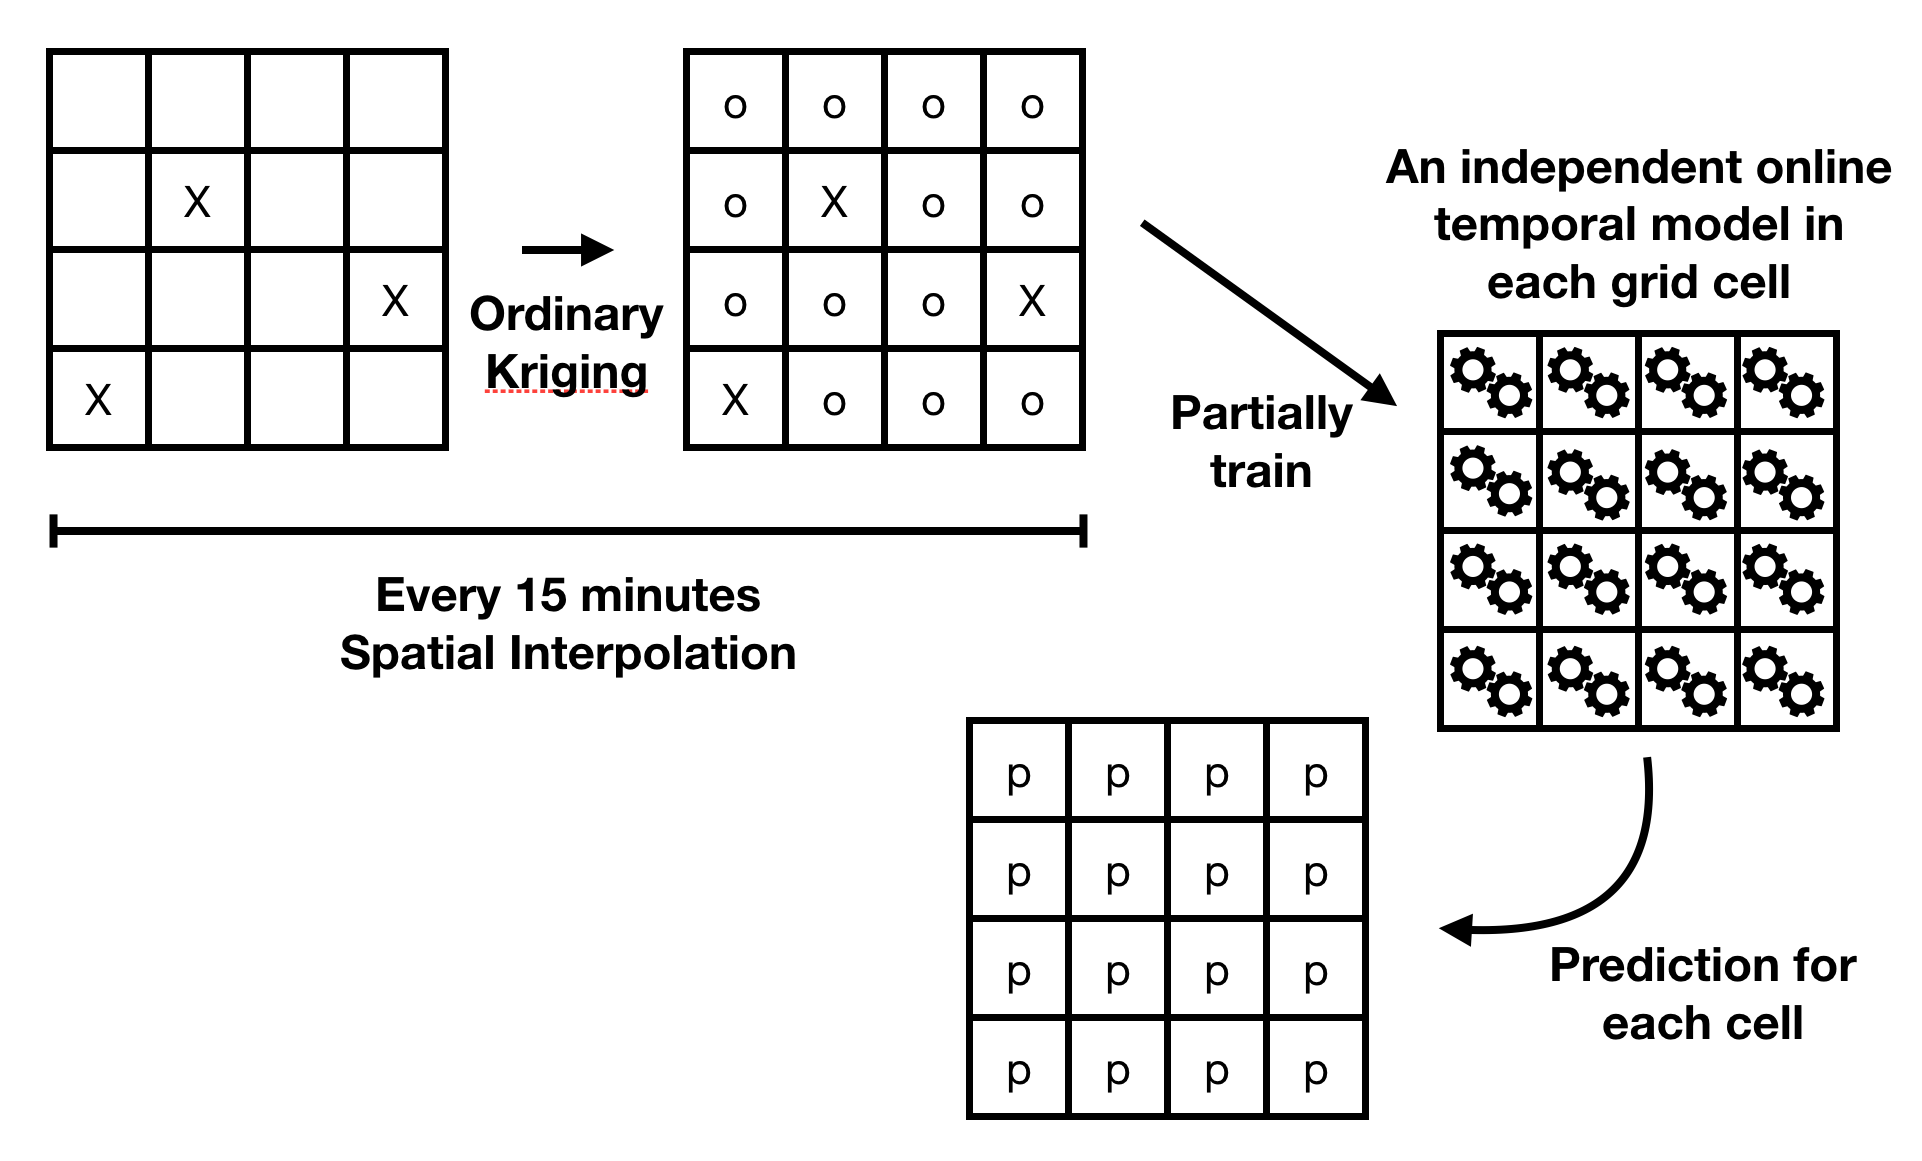
\includegraphics[width=\linewidth]{images/model_diagram.png} 
\caption{Online spatio-temporal model diagram. "X" denotes the cells where data was collected either with stationary or mobile sensors. "o" denotes the values interpolated from the cells with "X".}
\label{fig:model_diagram}
\vspace{1cm}
\end{figure}

\begin{figure}[H]
\centering
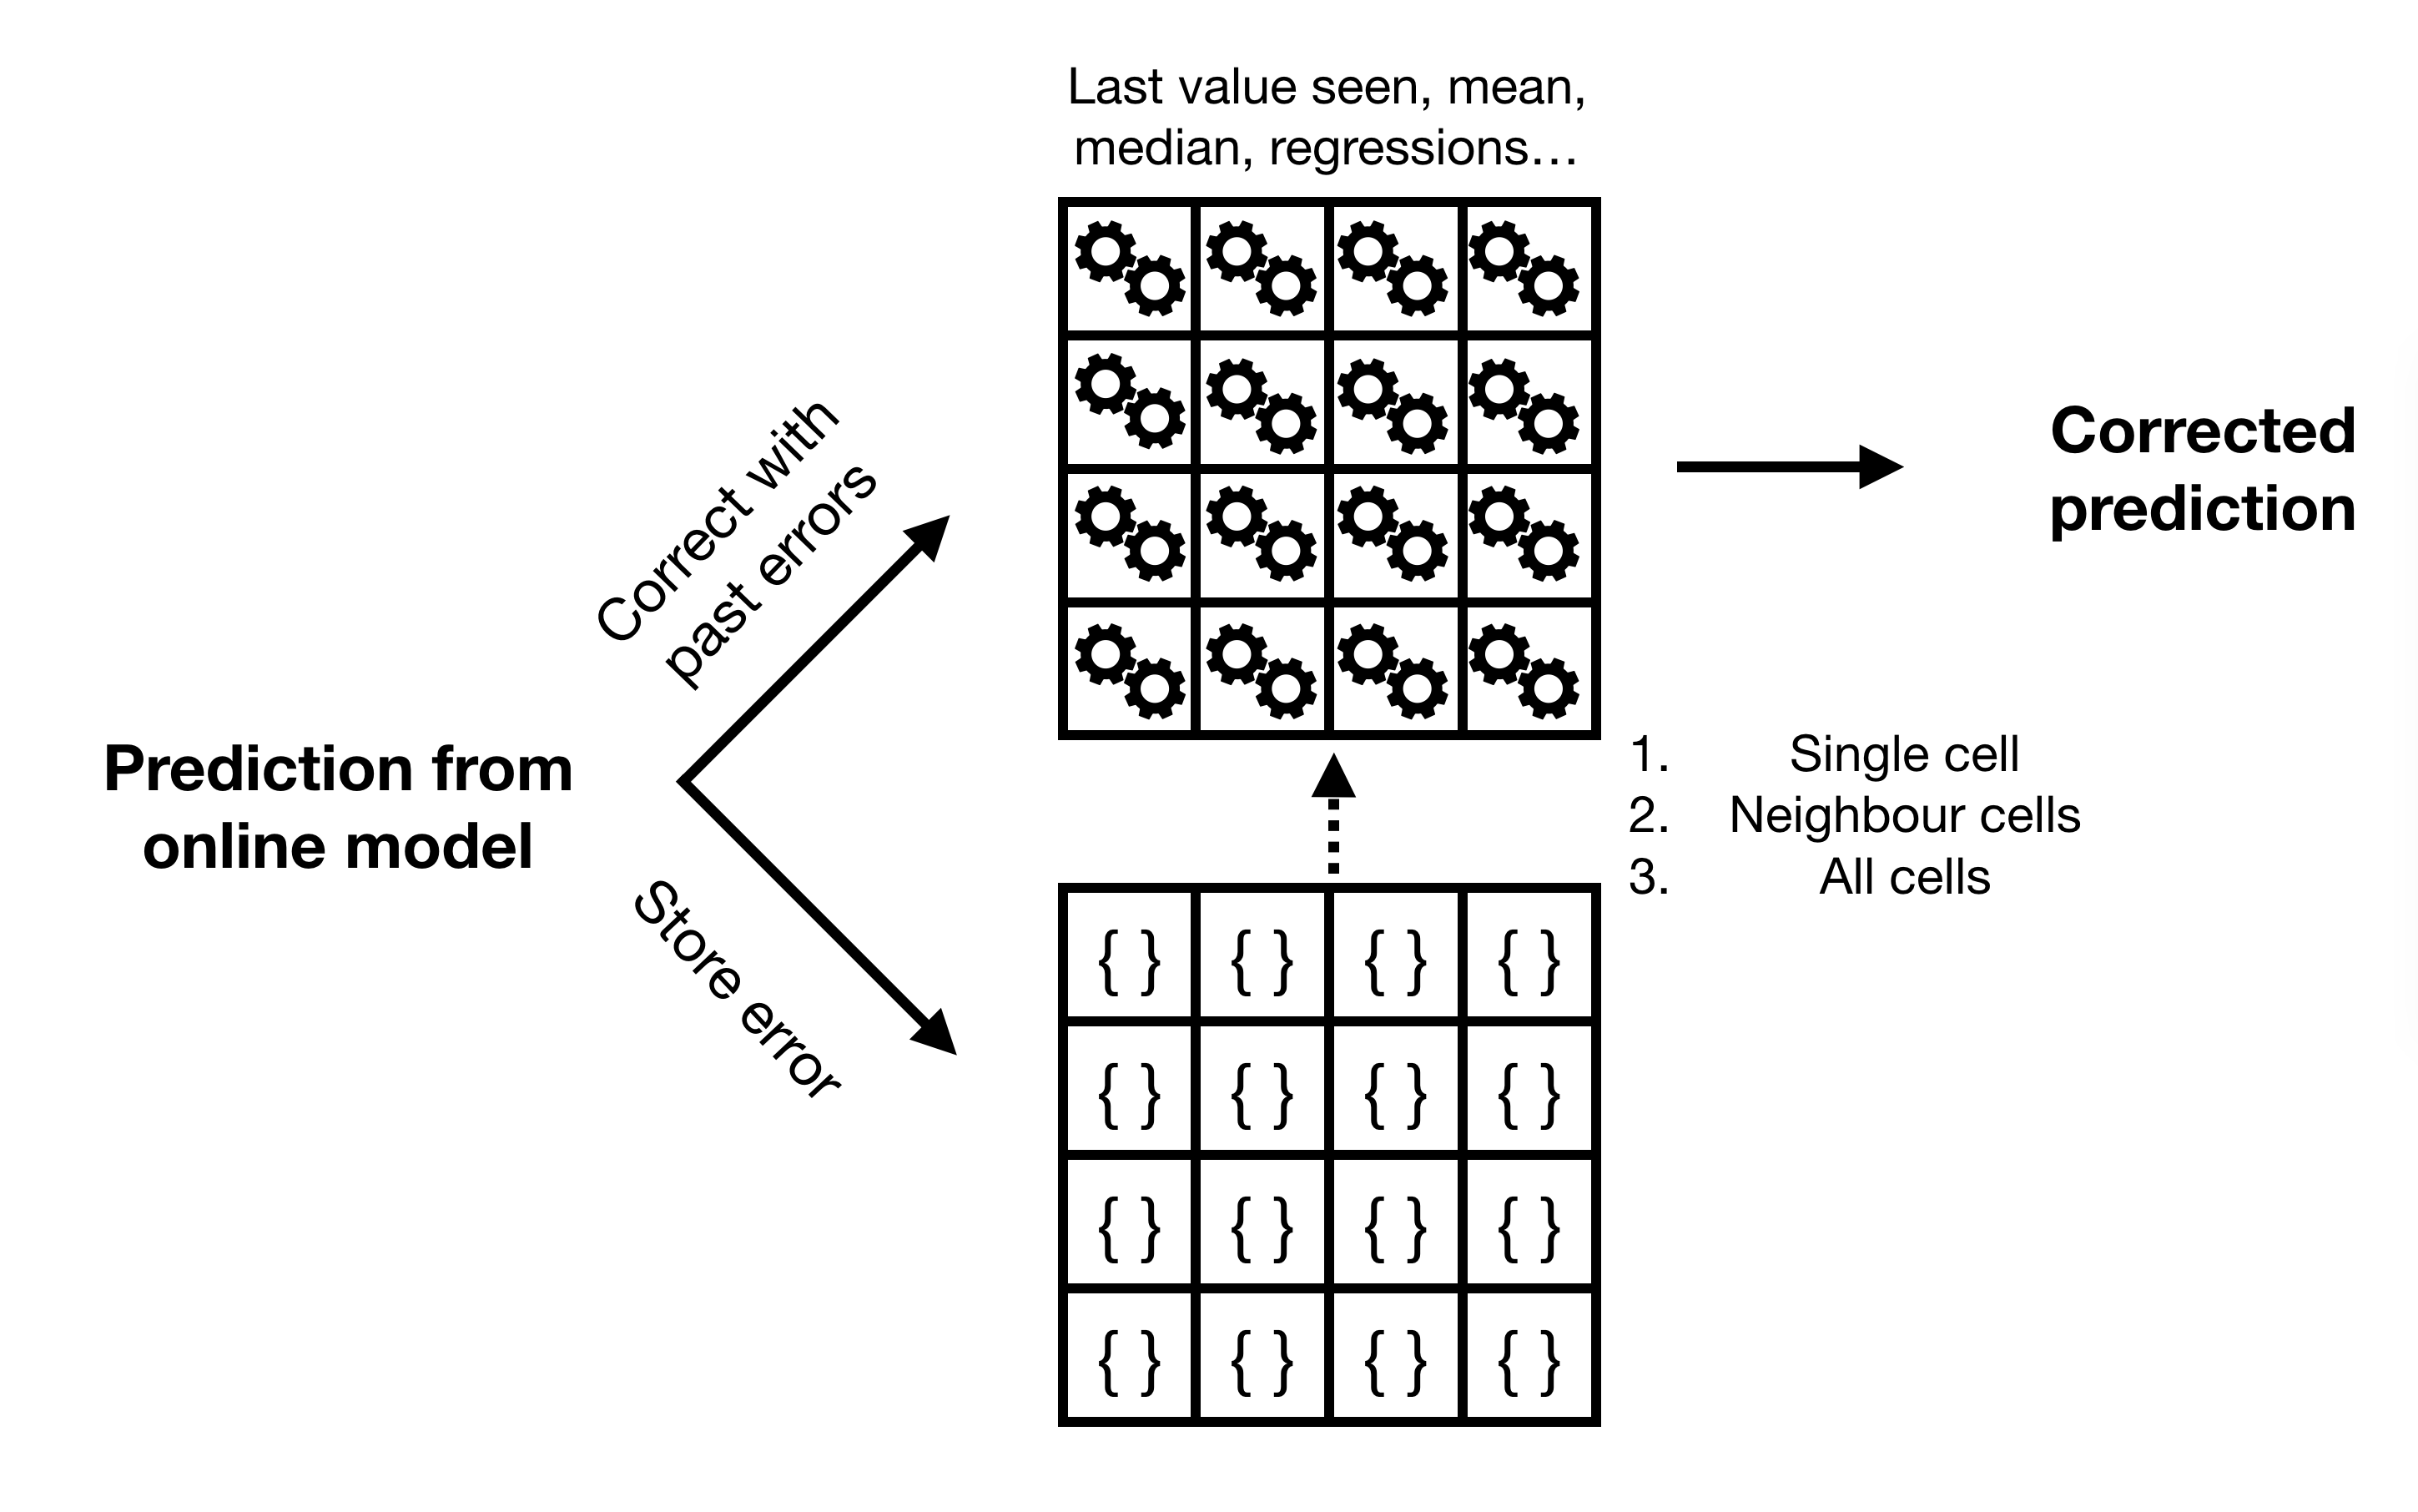
\includegraphics[width=\linewidth]{images/error_correction_diagram.png} 
\caption{Error correction algorithm diagram}
\label{fig:error_diagram}
\end{figure}

The error calculation is detailed in Figure \ref{fig:delta_correction}. The error is the difference between the prediction made in the past and the ground truth seen at the time corresponding to the prediction goal.  That error is stored in a data structure for correction of future predictions, along with the location and time of the occurrence.

\begin{figure}[H]
\centering
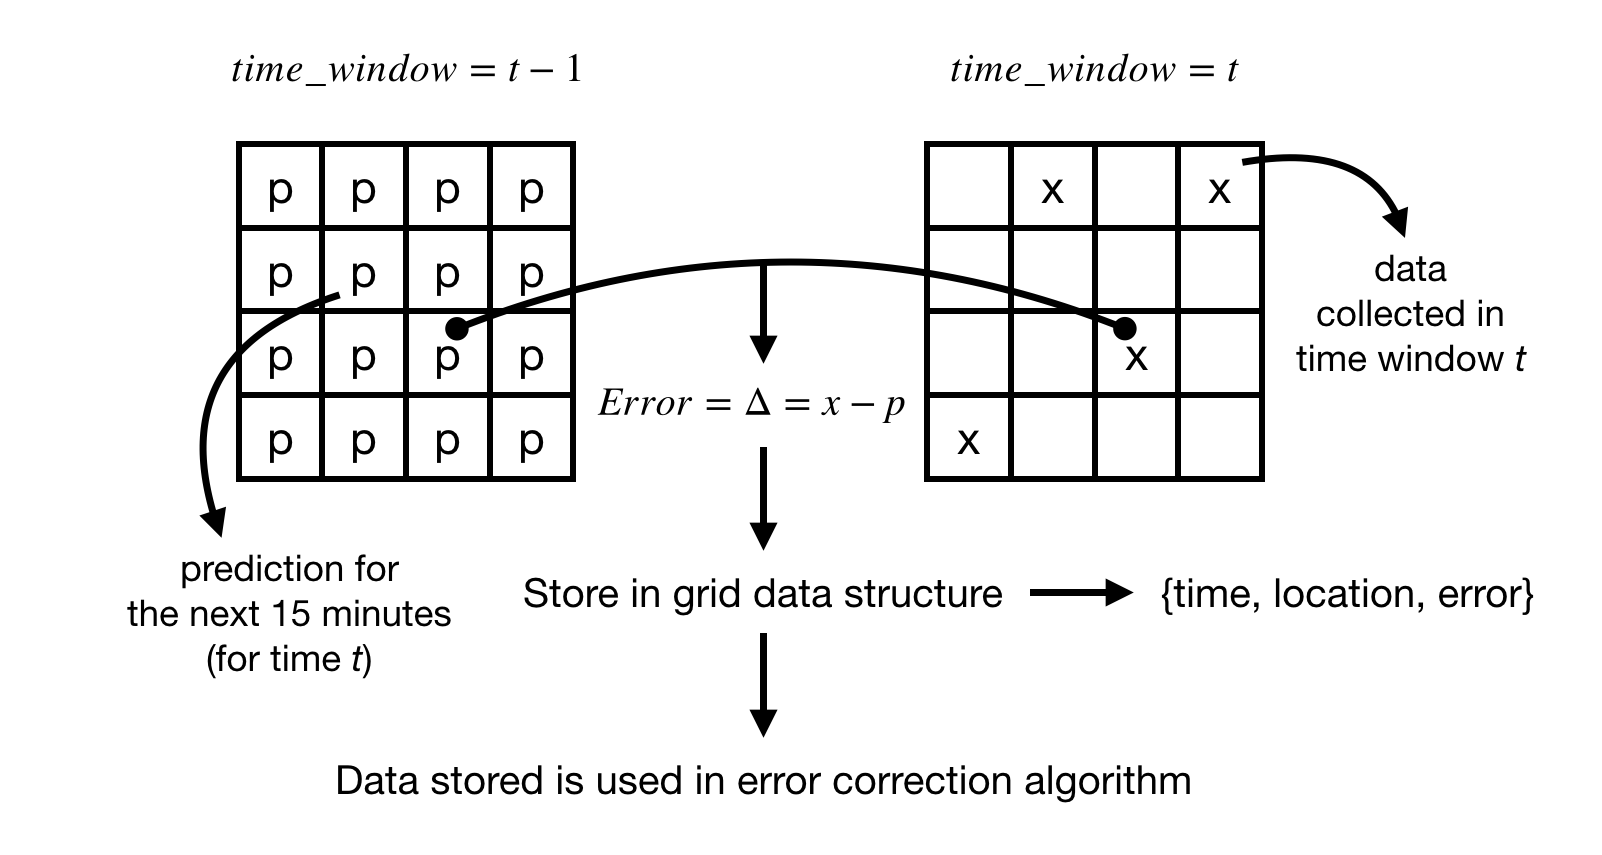
\includegraphics[width=\linewidth]{images/delta_correction.png} 
\caption{Error computation and storage diagram}
\label{fig:delta_correction}
\vspace{1cm}
\end{figure}


\section{Performance metrics}
The model was evaluated using several metrics on different test sets, depending on the experiment. The ground truth values used were the values read in the timestep that the prediction aimed for in the future. Therefore, only cell grids with values read in the future (after the simulated present of the model) can be used to measure the performance of the model.
Consider $O$ the observed value collected by the sensors and $P$ the predicted value (output of the model). Also, consider error $E$ as the difference between the ground truth and the predicted value ( $E = O-P$ ). The absolute error $AE$ is, therefore, the absolute value of the error ($AE = \mid O-P \mid$).
Mean Absolute Error (MAE) was the most used metric used to evaluate the performance of the model. Mean Absolute Error, described as the average of the Absolute Errors, has the same unit as the original data and can be simply defined by:

\[MAE = \frac{\sum_{i=1}^{n} AE_i}{n} = \frac{\sum_{i=1}^{n} \mid E_i \mid}{n} = \frac{\sum_{i=1}^{n} \mid O_i-P_i \mid}{n}\]

MAE ranges from 0 to $\infty$ and the lower the value, the better the model being evaluated.

Root Squared Error (RSE) is a similar metric that gives more weight to higher errors because these are squared. The same amount of absolute error divided over several observations and predictions would yield a lower RSE than the same absolute error observed in a single observations and prediction. RSE is similarly defined by: 

\[RSE = \frac{\sum_{i=1}^{n} E_i^2}{n} = \frac{\sum_{i=1}^{n} (O_i-P_i)^2}{n}\]

The lower the RSE, the better the model performance is. Lastly, Root Mean Square Deviation (RMSE), also referred to as Root Mean Square Error (RMSE) is the square root of RSE, therefore behaves similarly to it. The lower the RMSE, the better the performance.


\section{Baselines}
\label{chap:baselines}

Two types of baselines were used to compare and evaluate the predictions: one purely on the temporal basis and another one on the spatio-temporal basis.
The temporal baseline can only be applied in the cell grids with stationary sensors as these are the only ones that have continuous data in the temporal dimension.
Comparable work performed by Ivan Angelinin and Mantas Miksys used the value read 24 hours before and an RMSD of 5 respectively as the temporal baseline.
However, in addition to these benchmarks, two new baselines were developed, which performed better than the previous ones. The new baselines correspond to using the past 60 minutes or the last 15 minutes to predict the value. These are predictions that include more recent data observed, and because the data is temporally closer to what is trying to be predicted, better results were expected. Table \ref{tab:tempbaselines} shows the results of the temporal baseline applied to dataset A.

\begin{table}[h]
\centering
\begin{tabular}{c|ccc}
\textbf{} & \textbf{\begin{tabular}[c]{@{}c@{}}Mean Absolute \\ Error\end{tabular}} & \textbf{\begin{tabular}[c]{@{}c@{}}Mean Squared\\ Error\end{tabular}} & \textbf{\begin{tabular}[c]{@{}c@{}}Root Mean \\ Square Deviation\end{tabular}} \\ \hline
Ivan Angelinin's Baseline & 0.65 & 1.01 & 1.00 \\ \hline
Mantas Miksys' Baseline & - & - & 5 \\ \hline
60 minute Basline & 0.25 & 0.15 & 0.39 \\ \hline
\textbf{\begin{tabular}[c]{@{}c@{}}15 minute  Baseline\\ (proposed baseline)\end{tabular}} & 0.16 & 0.08 & 0.28 \\ \hline
\end{tabular}
\caption{Temporal Baselines Results}
\label{tab:tempbaselines}
\end{table}

The second type of baseline used is a spatio-temporal baseline. The best baseline found consists of predicting the PM2.5 concentration level in a cell grid at a specific timestep by using the most recent value read in the closest stationary sensor available. This baseline yielded the following results for dataset A:
\begin{itemize}
  \item Mean Absolute Error: 2.81
  \item Root Mean Squared Error: 3.87
\end{itemize}
The model outperformed the baseline model regardless whether or not error correction was used (see \autoref{chap:st_results}).



\chapter{Results and discussion}
\section{Temporal Results and Analysis}

\subsection{Hyperparameter Optimization}
The grid of Passive-Aggressive Regressor models that perform the temporal predictions have several hyperparameters that need optimization to fit better with the application and obtain better results. Only data from static sensors of dataset A was used for optimization. The approach used was grid search across three different variables: C, epsilon and loss as explained in section \ref{chap:par} and the values experimented are listed in Table \ref{tab:hyperparams}.

\begin{table}[H]
\centering
\resizebox{\textwidth}{!}{%
\begin{tabular}{|c|c|c|}
\textbf{Hperparameter "C"} & \textbf{Hyperparameter "epsilon"} & \textbf{Hyperparameter "loss"} \\
\multicolumn{1}{|l|}{} & \multicolumn{1}{l|}{} & \multicolumn{1}{l|}{} \\
$\num{2e-7}$ & $\num{1e-3}$ & squared\_epsilon\_insensitive \\
$\num{2e-5}$ & $\num{1e-1}$ & epsilon\_insensitive \\
$\num{2e-4}$ & $\num{5e-1}$ &  \\
$\num{2e-3}$ & 1 &  \\
$\num{2e-2}$ & 2.5 &  \\
$\num{2e-1}$ & 5 &  \\
2 &  & 
\end{tabular}%
}
\caption{List of hyperparameters used in grid search method}
\label{tab:hyperparams}
\end{table}

The experiment was done independently for each static sensor in order to investigate if there were benefits of having independently adjusted hyperparameter settings for each cell or if the same configuration could be used throughout the grid. Purely from a programming perspective, the same set of hyperparameters in all cells would be a better design decision as it provides simplicity to the model and helps define hyperparameters in grid cells where not enough data is available, or data does not exist at all. As results demonstrate in Table \ref{tab:hyperresults}, there is a minimal improvement of performance when a different set of hyperparameters is applied to each square compared to having the same set of hyperparameters in the whole grid, 0.158 and 0.159 respectively.
This experiment demonstrated the best set of hyperparameters to be $C= \num{2e-5}$, $epsilon = 0.001$ and $loss = epsilon\_insensitive$.

In a real-time context, it could be useful to recompute the hyperparameters of the model from time to time to adapt to possible changes due to long term seasonal changes in the environment.

\begin{table}[h]
\centering
\resizebox{\textwidth}{!}{%
\begin{tabular}{c|c|c|c|c|c}
\textbf{Sensor Name} & Best C value & Best epsilon value & Best loss value & \textbf{Mean Absolute Error} & \multicolumn{1}{l}{\textbf{Mean Squared Error}} \\ \hline
Lauriston & $\num{2e-5}$ & 0.001 & epsilon\_insensitive & 0.125 & 0.031 \\
Melville & $\num{2e-5}$ & 0.1 & epsilon\_insensitive & 0.400 & 0.296 \\
Tennis Court & 0.2 & 0.001 & epsilon\_insensitive & 0.076 & 0.013 \\
Library & $\num{2e-5}$ & 0.001 & epsilon\_insensitive & 0.122 & 0.035 \\
Bristo Square & 2 & 0.001 & epsilon\_insensitive & 0.114 & 0.036 \\
Buccleuch Place & 2 & 0.001 & epsilon\_insensitive & 0.108 & 0.021 \\ \hline
\textbf{Average} & - & - & - & \textbf{0.158} & \textbf{0.072} \\ \hline
\textbf{\begin{tabular}[c]{@{}c@{}}Best values\\ for all sensors\end{tabular}} & \textbf{$\num{2e-5}$} & \textbf{0.001} & \textbf{epsilon\_insensitive} & \textbf{0.159} & \textbf{0.076} \\ \hline
\end{tabular}%
}
\caption{Grid search results}
\label{tab:hyperresults}
\end{table}

\subsection{Features of PAR model}
The results presented in Table \ref{tab:hyperresults} refer to a PAR model that only includes time as an input feature. However another set of features was experimented: one that included temperature, humidity and last PM2.5 value as features. The same hyperparameter optimization was executed (except attempt with $C=\num{2e-7}$). That experiment yielded a minimum MAE of $0.769$ and MSE of $1.21$, in the case $"C"= \num{2e-5}$, $"epsilon" = 0.5$ and $"loss" = epsilon\_insensitive$. Because of these results, this model was not explored further and the other model was used as the temporal model.

\subsection{Data noise reduction}

Figure \ref{fig:resamples} shows the data collected from one static sensor, resampled at different time durations. These four figures show the data noise is reduced as the time window size increases. Experiments were performed to investigate if noise reduction could improve the performance of the Passive-Aggressive Regressor, by increasing the time window. The results of using a 60-minute time window with a 45-minute overlap are displayed in Figure \ref{tab:distance_pred} and compared to the more straightforward 15 minute time window.

\begin{figure*}
\centering

\begin{subfigure}[t]{0.5\textwidth}
\centering
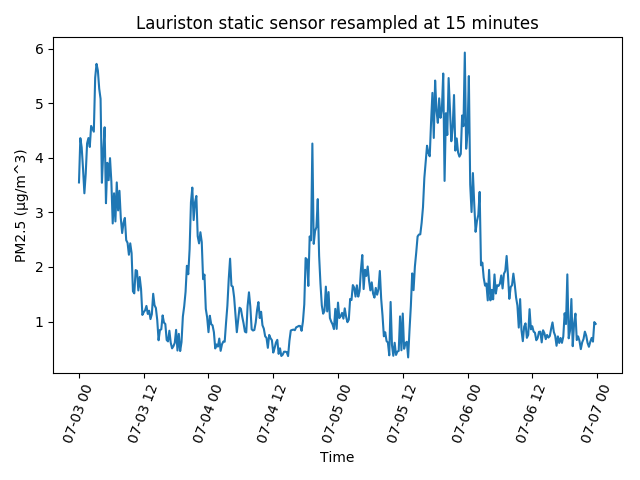
\includegraphics[width=\textwidth]{images/static_sensor_lauriston_resampled_15_min.png}
\caption{Values resampled to 15 minutes}
\label{fig:resample_15}
\end{subfigure}%
%
\hfill
%
\begin{subfigure}[t]{0.5\textwidth}
\centering
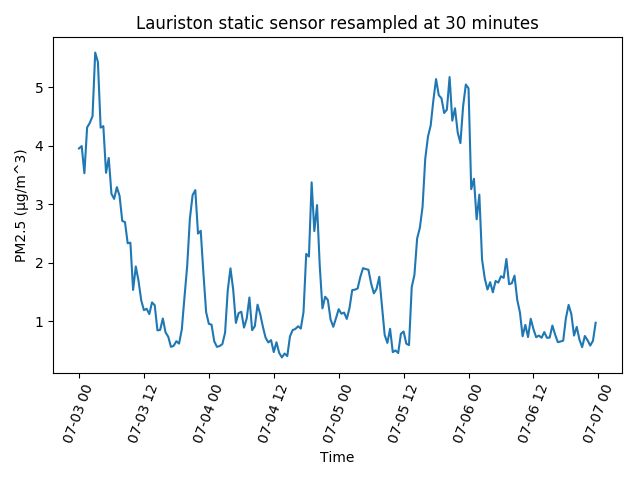
\includegraphics[width=\textwidth]{images/static_sensor_lauriston_resampled_30_min.png}
\caption{Values resampled to 30 minutes}
\label{fig:resample_30}
\end{subfigure}

\bigskip 

\begin{subfigure}[t]{0.5\textwidth}
\centering
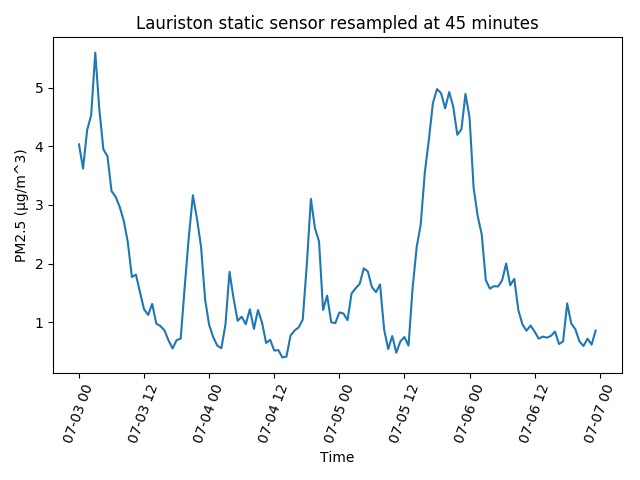
\includegraphics[width=\textwidth]{images/static_sensor_lauriston_resampled_45_min.png}
\caption{Values resampled to 45 minutes}
\label{fig:resample_45}
\end{subfigure}%
%
\hfill
%
\begin{subfigure}[t]{0.5\textwidth}
\centering
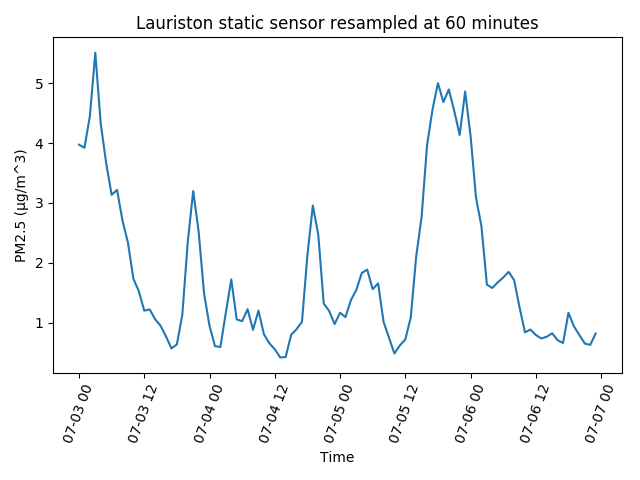
\includegraphics[width=\textwidth]{images/static_sensor_lauriston_resampled_60_min.png}
\caption{Values resampled to 60 minutes}
\label{fig:resample_60}
\end{subfigure}

\caption{Lauriston static sensor readings on dataset A}
\label{fig:resamples}
\end{figure*}


\begin{table}[h]
\centering
\resizebox{\textwidth}{!}{%
\begin{tabular}{c|c|c}
\textbf{Training method (MAE/MSE)} & \textbf{Predicting 15 minutes ahead} & \textbf{Predicting 60 minutes ahead} \\ \hline
Using 15 minute intervals & \textbf{0.159 / 0.076} & 0.254 / 0.156 \\ \hline
\begin{tabular}[c]{@{}c@{}}Using a 60-minute rolling mean every 15 minutes \\ (45 minutes overlap)\end{tabular} & 0.180 / 0.078 & 0.291 / 0.182
\end{tabular}%
}
\caption{MAE and MSE comparison of time windows and prediction distance}
\label{tab:distance_pred}
\end{table}

Results show that regardless of the prediction distance, 15 minutes ahead or 60 minutes ahead, using the 15 minute time window performs better than using a 60-minute rolling mean. It is also possible to observe that predicting 15 minutes into the future produces less error than 60 minutes ahead, as would be expected.

Figure \ref{fig:errorahead} illustrates the comparison of errors when only predictions are made (blue line) and when predicting and training is occurring (orange line). The blue line corresponds to the online model proposed because, at every step in the horizontal axis, the model is partially trained with the data seen in the window before. In contrast, the orange line shows the error increasing over time as the model was only trained at time window zero and the model tries to predict further into the future without the knowledge of the most recent data. In this Figure, we can observe the advantages of the online model to make shorter-term predictions, as the capability to adapt to very recent data by partially training more frequently allows the error to remain low over time.

\begin{figure}[h]
    \centering
    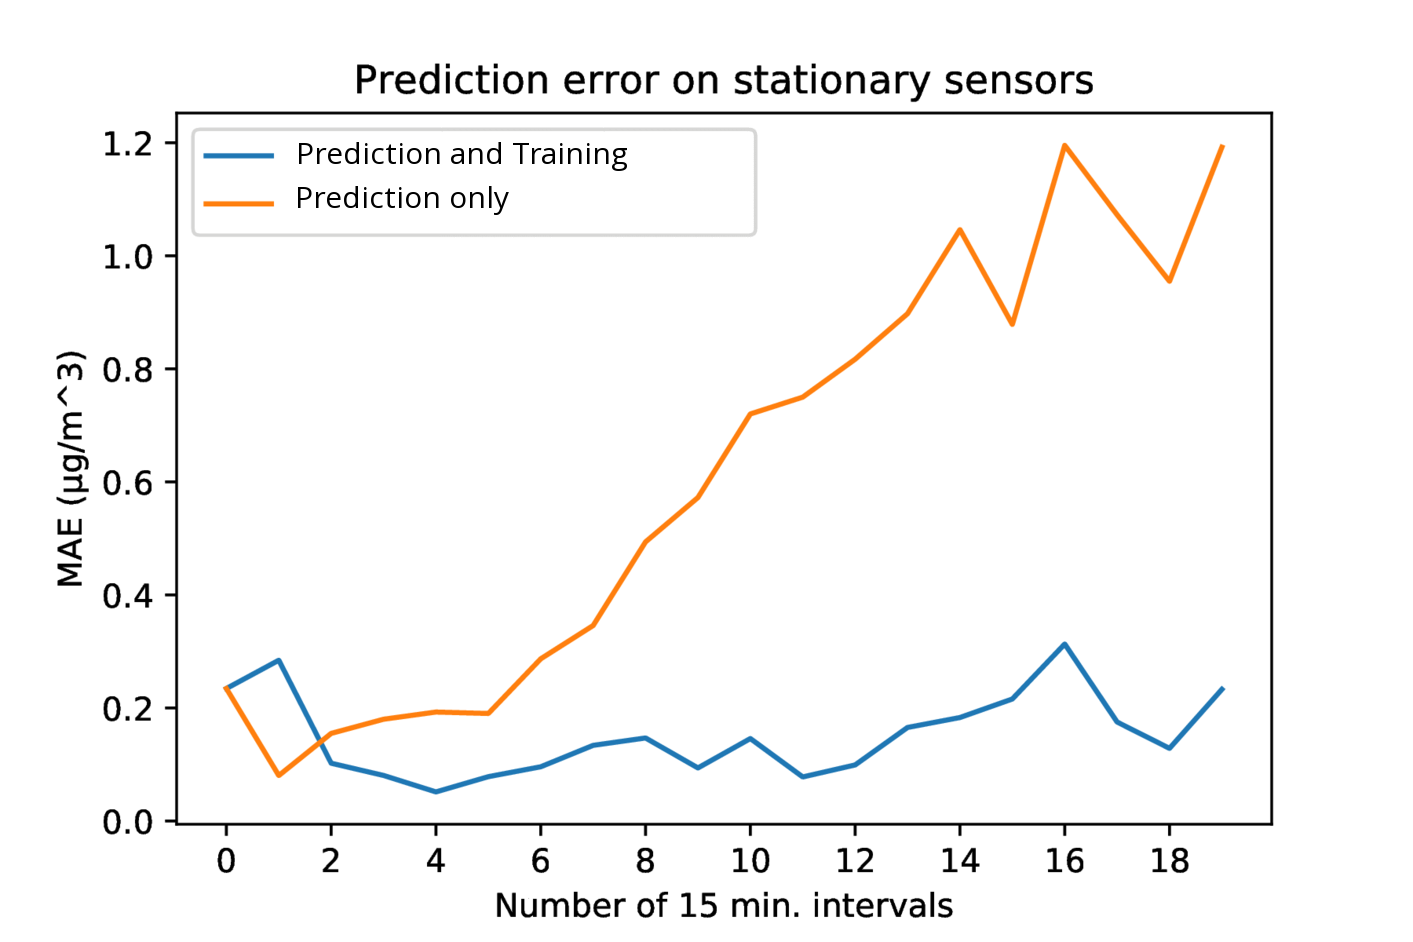
\includegraphics[width=0.8\textwidth]{images/prediction_error.png}
    \caption{Comparison between only predicting and predicting \& training (online) over time}
    \label{fig:errorahead}
\end{figure}

\section{Spatio-temporal Results and Analysis}
\label{chap:st_results}

The performance of the online spatio-temporal model is presented in this section. One of the novel parts of the model, the integration of mobile data in the online training phase of the model was compared to the model without mobile data included in the training. Tests were made by comparing the predictions with the values read in the corresponding time window and cell grid. Both datasets, A and B, were tested. Overfitting to the training set does not apply in this case as the ground truth of a prediction is data that the model has not yet seen given it is a time in the future (future of where the model is simulated to be). Results were summarised in Table \ref{tab:spatiotemporal}. The analysis of these results shows that including mobile data in training the model improves predictions by $14\%$ in dataset A and $20\%$ in dataset B. 
This improvement in performance can also be attributed to the fact that the data that is being tested is geographically close to observations that were known shortly before and the online model was able to adapt to them, making use of locality to improve predictions. As an example, imagine a person walking a path throughout the grid with a mobile sensor reading PM2.5 values. The values that person collected 15 minutes before the present will be spatially close to where the person is located in the present, and because the model was able to adapt quickly to the data collected 15 minutes ago, the predictions to that person are improved in the present.
It is also important to refer from Table \ref{tab:spatiotemporal} that the results are 19\% better than the baseline in dataset A defined in section \ref{chap:baselines} as 2.81.

Note that the model supports data of mobile sensors regardless of the way they were collected, such as walking, cycling, skating, and more. The locality advantage still applies in these cases because from the model's perspective the only change that occurs is the number of cell grids travelled in each time window, and consecutive time windows share nearby observed grid cells. In the datasets used, both walking and cycling data were available and used.

It is also possible to analyse these results from another perspective. Given that the MAE of the temporal model achieved on cells with static sensors in place is $0.159$ (from \ref{tab:distance_pred}), and the MAE of the spatio-temporal model on cells where mobile data was collected is $2.28$ (from \ref{tab:spatiotemporal}), we could extract two insights about the data: Firstly, would it be the case where the whole grid is filled with static sensors or data for all grid cells is available through static and mobile sensors, we could see the spatio-temporal MAE get closer to the temporal MAE. Secondly, we can identify the spatial interpolation as a significant source of error. Further experiments described in section \ref{improvement} try to improve that performance with success.



\begin{table}[H]
\centering
\resizebox{\textwidth}{!}{%
\begin{tabular}{c|c|l|c|l|}
\textbf{Training method} & \multicolumn{2}{c|}{\textbf{Dataset A}} & \multicolumn{2}{c|}{\textbf{Dataset B}} \\ \cline{2-5} 
\multicolumn{1}{l|}{} & \multicolumn{1}{l|}{\textbf{With mobile data}} & Without mobile data & \multicolumn{1}{l|}{\textbf{With mobile data}} & Without mobile data \\ \hline
Number of squares tested & \multicolumn{2}{c|}{369} & \multicolumn{2}{c|}{301} \\ \hline
Mean Absolute Error & \textbf{2.28} & \multicolumn{1}{c|}{2.65} & \textbf{1.21} & \multicolumn{1}{c|}{1.51} \\ \hline
\end{tabular}%
}
\caption{Spatio-temporal MAE results and Analysis}
\label{tab:spatiotemporal}
\end{table}

\subsection{Error visualisation}
In order to reduce the error, a script was developed to visualise the errors of the model. The result is presented in Figure \ref{fig:error_st}. In this Figure, it was detected that errors were mostly positive, indicating the model was mostly underpredicting the PM2.5 levels. If the model was not underpredicting, the green line, representing the mean of the errors would be on or close to zero, the red line drawn in the graph. That is not the case and indicates an improvement in accuracy could be achievable.


\begin{figure}[H] 
\centering
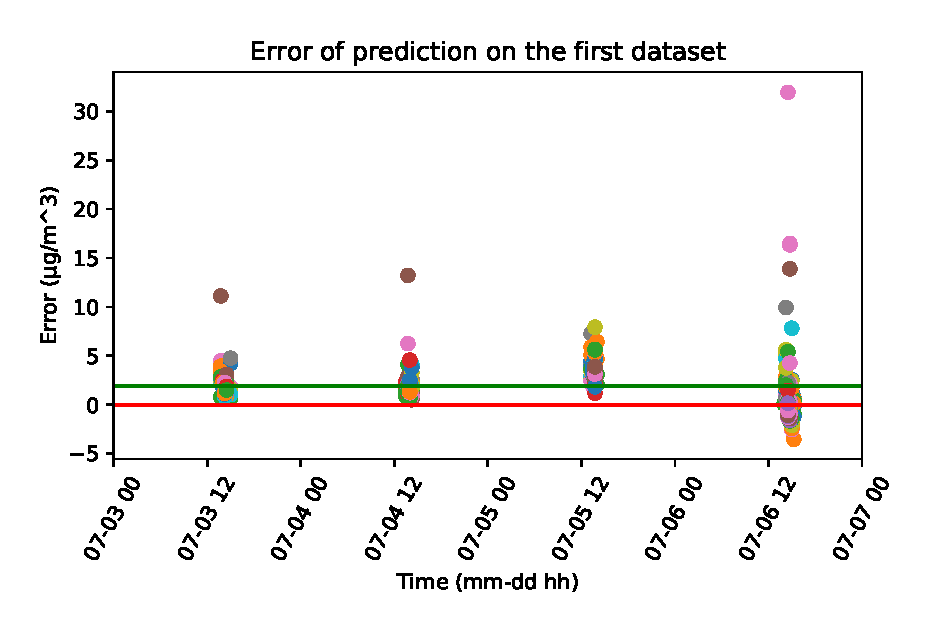
\includegraphics[width=\linewidth]{images/daily_error_with_line.eps} 
\caption{Errors of spatio-temporal model on dataset A. Different coloured dots represent the errors of the predictions made. The red line is defined as $Error = 0$ and the green line is defined by $Error = \textrm{\textit{Average of all errors displayed}} = 1.87 $.}
\label{fig:error_st}
\end{figure}

\section{Improvement using bias correction}
\label{improvement}

Using the known tendency for the model to underestimate predictions, an online correction system was produced to counter this imbalance. This aimed to further improve the performance of the prediction system without compromising the capability for the model to adapt in a real-time context.
The tests with the data correction algorithm were performed on dataset B, having dataset A just as training data to compute initial prediction errors. As seen in Figure \ref{fig:hist_mobile}, the mobile data available is sparse, and this method prevents a cold start of the algorithm. 
The correction algorithm's performance is compared to the base model performance without the algorithm in place. The aim is to achieve better performance than the base model, which, on dataset B produced MAE of 1.21.
Several experiments were implemented to analyse the improvement in performance on the base model. Three parameters were tested: The minimum amount of data stored to activate the error correction, the radius of the errors considered in the computation and the method of computing the amount of correction. 

Firstly, the minimum amount of data to prevent a cold start was tested, and results are presented in Table \ref{tab:min_threshold}. It is observable that the results remain relatively constant as the threshold increases and after that, when the threshold is big enough not to activate very often, the MAE gets closer to the MAE value without correction applied. Effectively, if a big enough threshold was chosen, the error correction would never activate and error output would be the same as the model without correction. There were no significant differences in setting the minimum amount of data needed to correct the prediction, therefore, a minimum of 3 errors was therefore chosen.

\begin{table}[]
\centering
\resizebox{\textwidth}{!}{%
\begin{tabular}{l|c|l|l|l}
 & \multicolumn{4}{c|}{Experiment performed with method "mean" and local data only} \\ \hline
 & \multicolumn{1}{l|}{\textbf{Minimum threshold = 3}} & Minimum threshold = 5 & Minimum threshold = 7 & \multicolumn{1}{l|}{Minimum threshold = 10} \\ \hline
\multicolumn{1}{c|}{Mean Absolute Error} & \textbf{1.293} & \multicolumn{1}{c|}{1.294} & \multicolumn{1}{c|}{1.294} & \multicolumn{1}{c|}{1.241} \\ \hline
\end{tabular}%
}
\caption{Minimum activation threshold experiment results}
\label{tab:min_threshold}
\end{table}

Secondly, three radii of data used for correction were tested. One where only data from the same cell would be used, referred to as using local data, one where adjacent cells would also be used, referred to as using neighbouring data and one where data from all cells would be used, referred to using global data. These three alternatives are represented in Figure \ref{fig:error_corrcections}.

\begin{figure}[h]
\centering
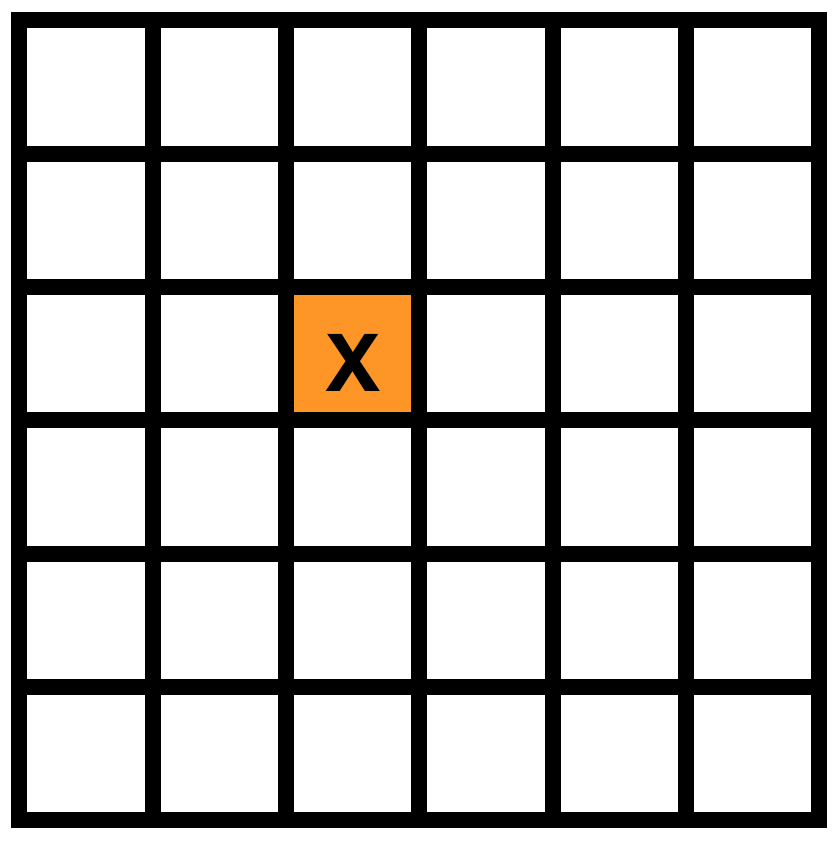
\includegraphics[width=.3\textwidth]{images/local_error.png}\hfill
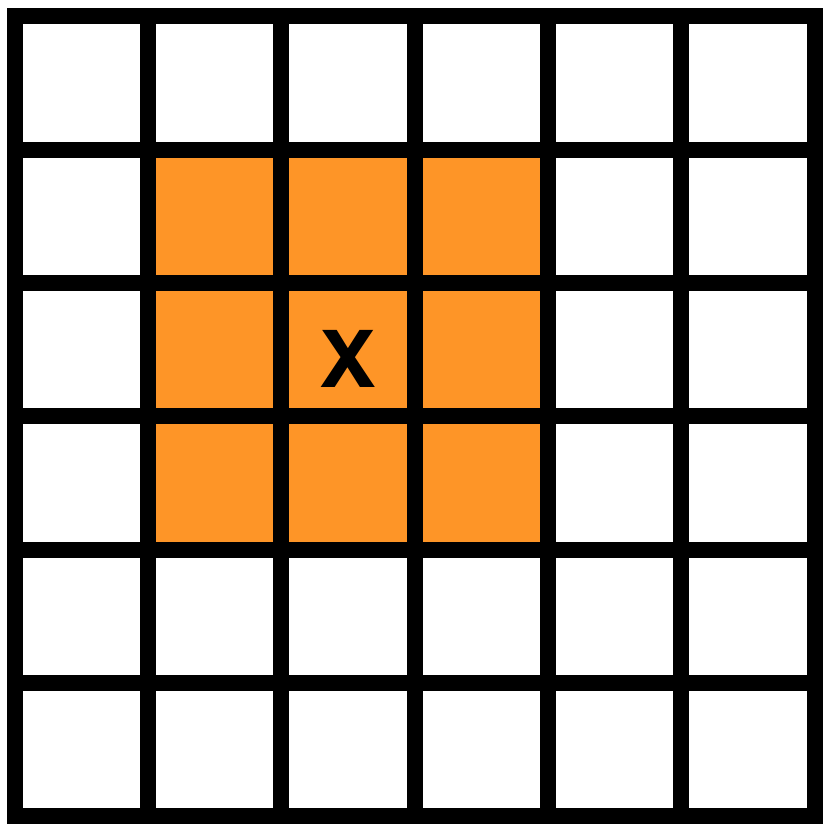
\includegraphics[width=.3\textwidth]{images/neighobour_error.png}\hfill
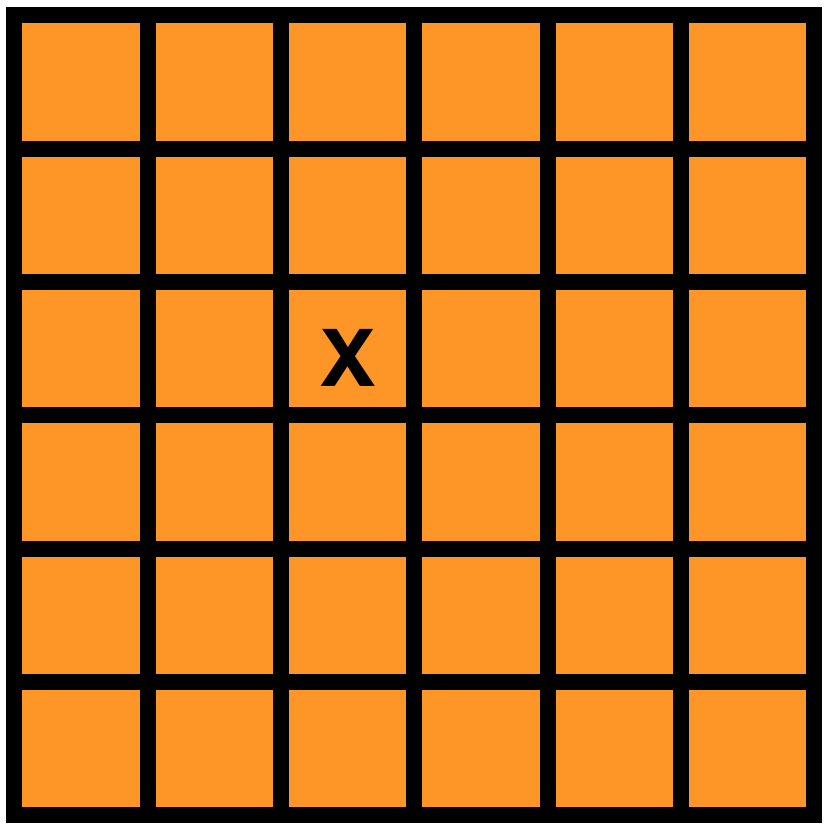
\includegraphics[width=.3\textwidth]{images/global_error.png}
\caption{Representation of errors used in local (left), neighboring (center) and global (right) scenarios, where "X" represents the location of the error correction that is being applied and orange filling represents the errors used to compute the error correction value.}
\label{fig:error_corrcections}

\end{figure}

\begin{table}[h]
\centering
\resizebox{\textwidth}{!}{%
\begin{tabular}{c|c|c|c|}
 & \multicolumn{3}{c|}{\begin{tabular}[c]{@{}c@{}}Experiment performed with minimum threshold = 3 \\ and mean as computation method\end{tabular}} \\ \hline
 & Local data & Neighboring data & \textbf{Global data} \\ \hline
Mean Absolute Error & 1.293 & 1.201 & \textbf{1.060} \\ \hline
\end{tabular}%
}
\caption{Results using different amounts of data for error correction}
\label{tab:mean_results}
\end{table}


The results of this experiment (Table \ref{tab:mean_results}) revealed that the error correction improvement is a very useful tool to make better predictions, but the tests show that there was not enough data on a small set of grid cells that allow the radius to be smaller than the entire grid. The more data is available in each cell, which is collected over time, the smaller the range can be and it would be interesting to investigate in the future whether this reduction of radius could even improve the predictions further, as each cell grid could have more detailed data about its specific behaviour in terms of errors.



Lastly, several methods of computing the amount of correction were tested: statistical properties such as mean and median, most recent error selection, and regression models such as linear regression and passive-aggressive regressor. Inspection of Table \ref{tab:local_global} shows that the machine learning models don't have enough data to be able to compare with statistical models, however, the Linear Regression model on global data was able to perform better than the model without correction even with the small amount of data. This indicates that, in the future, regression models could, with a more substantial amount of data data available, also improve the predictions, possibly even surpassing statistical models. Both the mean and the median methods were able to improve the performance of the predictions using global data, especially the median, which was the best performing correction method tested. This behaviour is likely to be due to the existence of outliers in dataset B, which the mean is more sensitive to than the median, making the median a more robust method to compute the correction to be applied. The error correction part of the model, therefore, improves performance by 22\% compared to the same model without error correction.

\begin{table}[h]
\centering
\resizebox{\textwidth}{!}{%
\begin{tabular}{c|c|c|}
 & \multicolumn{2}{c|}{Experiment performed with minimum threshold = 3} \\ \hline
Mean Abolute Error (MAE) & \multicolumn{2}{c|}{Data used} \\ \hline
Method of correction calculation & Local data & \textbf{Global data} \\ \hline
Last value seen & 1.452 & - \\
Mean & 1.293 & \textbf{1.060} \\
\textbf{Median} & 1.226 & \textbf{0.948} \\
Passive-Aggressive Regression & 6.212 & 3.700 \\
Linear Regression & 5.352 & \textbf{1.116}
\end{tabular}%
}
\caption{Comparison of different correction calculation methods. The results highlighted correspond to those that improve the model.}
\label{tab:local_global}
\end{table}




\chapter{Conclusion}
Air pollution and $PM_{2.5}$ particularly has been shown to have an impact on citizen's lives, especially those that have respiratory conditions such as asthma or chronic obstructive pulmonary disease. Intra-urban and short-term predictions can significantly help to inform and to warn people, guided by data-driven decision making, to avoid polluted areas and particulate matter exposure. The nature of air pollution dispersion is complex and dependent on many factors such as meteorological changes, traffic patterns, the dimension of particulates and topography.

Reference sensors, used by official environmental institutions, are used to produce air quality forecasts; however, the dynamics of intra-urban air pollution cannot be represented with data from a limited amount of expensive and accurate sensors. An alternative to this approach, used in this project, is to use a network of inexpensive stationary sensors distributed throughout the city and mobile sensors to complement that data collection. This approach allows new techniques and methods to model air pollution at a high-resolution level.

Previous work on the Sensing Spaces project focused on online, spatial and temporal models independently and mobile data had never been used to train the models. This work did not allow to have a system capable of responding to changes in the environment nor cope with the sparsity of mobile data temporal and spatially. This project proposes an approach that combines Ordinary Kriging and Passive-Aggressive Regressors to make a coupled online spatio-temporal model. This model can adapt with time and predict in areas where data has not been observed. However, the accuracy depends on the amount of data available, when and where it was collected, and how recent it is.

The datasets used in this project both include data from six stationary sensors and two mobile sensors, the latter not used simultaneously. Both datasets include data from four days in July 2018 and four mobile data collection periods at similar times of day, averaging 53 minutes of data per day.

This project has presented a model capable of predicting PM2.5 concentration in intra-urban environments using both stationary sensor data as well as data collected by mobile sensors. It was designed with a real-time context in mind, by predicting and training in real time. The model performs better than a batch learning algorithm given its ability to adapt as new data comes in.  An improved User Interface that allows media collection within the RESPeck android application was also developed and tested with ten participants. Photographs were the most collected type of media, followed by text comments, video clips and lastly audio samples.
The analysis was made with data from July 2018 collected in Edinburgh by ZP with six stationary sensors and two mobile sensors. The experiments demonstrate that time is a better feature for the temporal model than temperature, humidity and past PM2.5 values and that reducing the data noise using a rolling mean of 60 minute does not improve results. The PAR model used for temporal predictions achieved an MAE of 0.159 and MSE of 0.076 with hyperparameters $C= \num{2e-5}$, $epsilon = 0.5$ and $loss = epsilon\_insensitive$ on static data of dataset A, collected in Edinburgh. The spatio-temporal model achieved an MAE of 2.28 on dataset A (19\% better than baseline) and 1.21 on dataset B. 

Five error correction algorithms (last seen value, mean, median, linear regression and passive-aggressive regressor) were tested as methods to improve the prediction output. The regression models showed viability to improve predictions if enough data is made available, but statistical methods performed better with the data currently available. The best error correction algorithm found has a minimum threshold of 3 data points to activate, uses the median as computation method and uses errors of all cells (global data), which further improved the model to an MAE of 0.948 on dataset B, using dataset A as training data, a further 22\% improvement compared to the model without error correction.


\section{Future Work}

It would be interesting to explore the performance of the model when several mobile sensors are concurrently collecting data in the test area along with the stationary sensors, increasing the data available in all time windows and having more grid cells filled with data, reducing sparsity. It would also be interesting to investigate different time periods such as mornings and nights and the model's ability to react to short term patterns such as peak and off-peak hours and other pollution metrics such as $PM_1$ and $PM_{10}$. Further investigation could attempt to demonstrate a correlation between PM values and use that correlation as a feature to the model proposed.

Future work can also concern the application of the models developed to new datasets and possibly new regions such as a dataset from India or an area of a major city such as London. Data from the PHILAP Project is a good example where useful data will be generated. This data will also have corresponding RESpeck data (breathing data), so a more extensive analysis can be done in the Sensing Spaces project, such as how to make these predictions useful in people's daily lives. Besides, a bigger dataset can further extend the error correction methodology, and new results could be derived from the machine learning regressors to be compared with the statistical metrics used currently. 

Other ways of collecting mobile data could be explored to increase the amount of data in the test area, such as placing sensors on public transportation or distributing them to food delivery cyclists that work in unusual periods such as evenings and late night.

The models presented can be used in several applications that future work could cover such as the implementation of a warning system for people especially affected by air pollution, or the integration of this model with path planning algorithms. Moreover, the system can be used to monitor and track air pollution in real time, empowering emergency responders, such as firefighters, with a tool that could detect incidents and anomalies or the citizen's to make better decisions such as where to spend more time outside.  

Several students will be working on the Sensing Spaces project during summer 2019; therefore their work will also be useful for Part II of the project.




% use the following and \cite{} as above if you use BibTeX
% otherwise generate bibtem entries
\bibliographystyle{plain}
\bibliography{mybibfile}

\appendix
\chapter{}
\section{Information Sheet}
\label{sec:infosheet}


\begin{figure}[H]
\centering
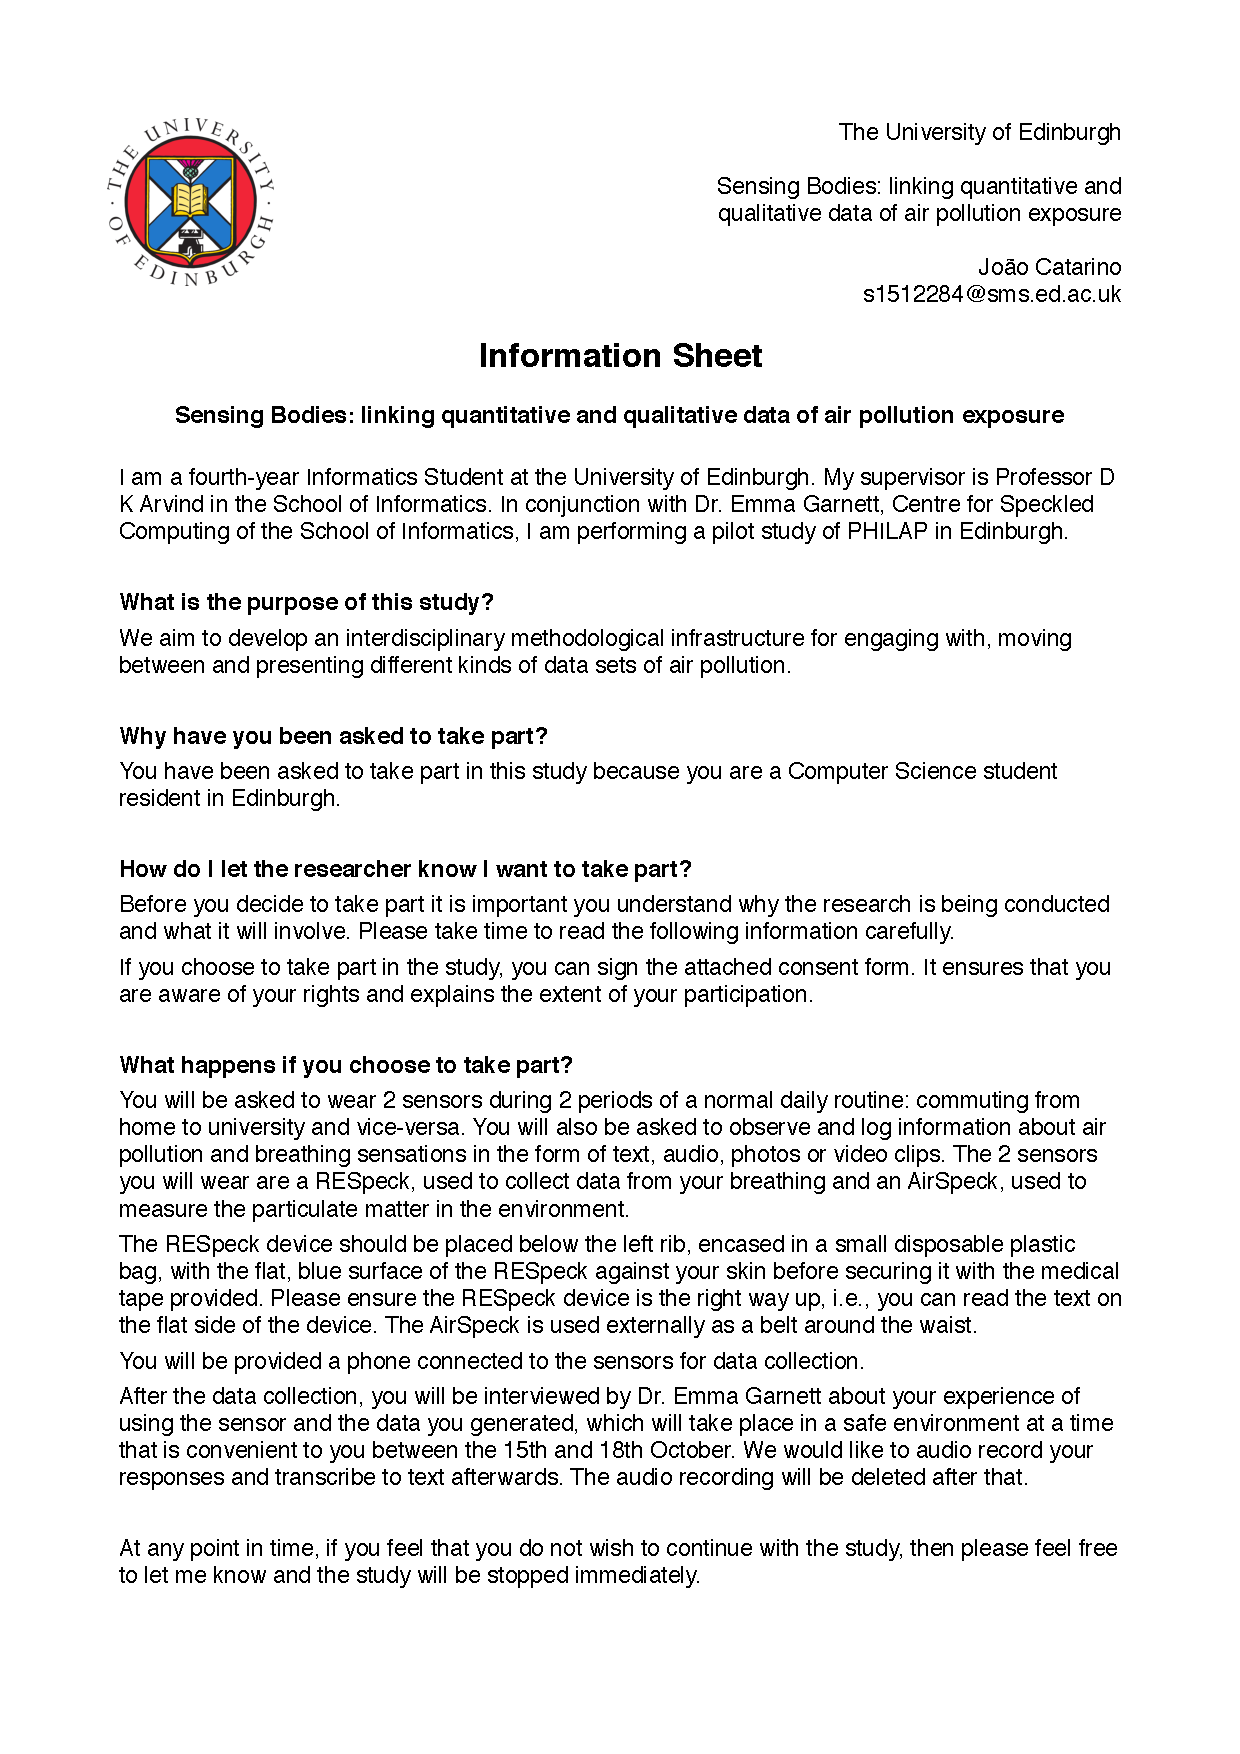
\includegraphics[width=.8\textwidth]{pdfs/information}
\caption{Participant Information Sheet (Page 1)}
\label{infosheet}
\end{figure}

\begin{figure}[H]
\centering
\includegraphics[width=\textwidth, page=2]{pdfs/information}
\caption{Participant Information Sheet (Page 2)}
\label{infosheet}
\end{figure}

\section{Consent Form}
\label{sec:consent}

\begin{figure}[H]
\centering
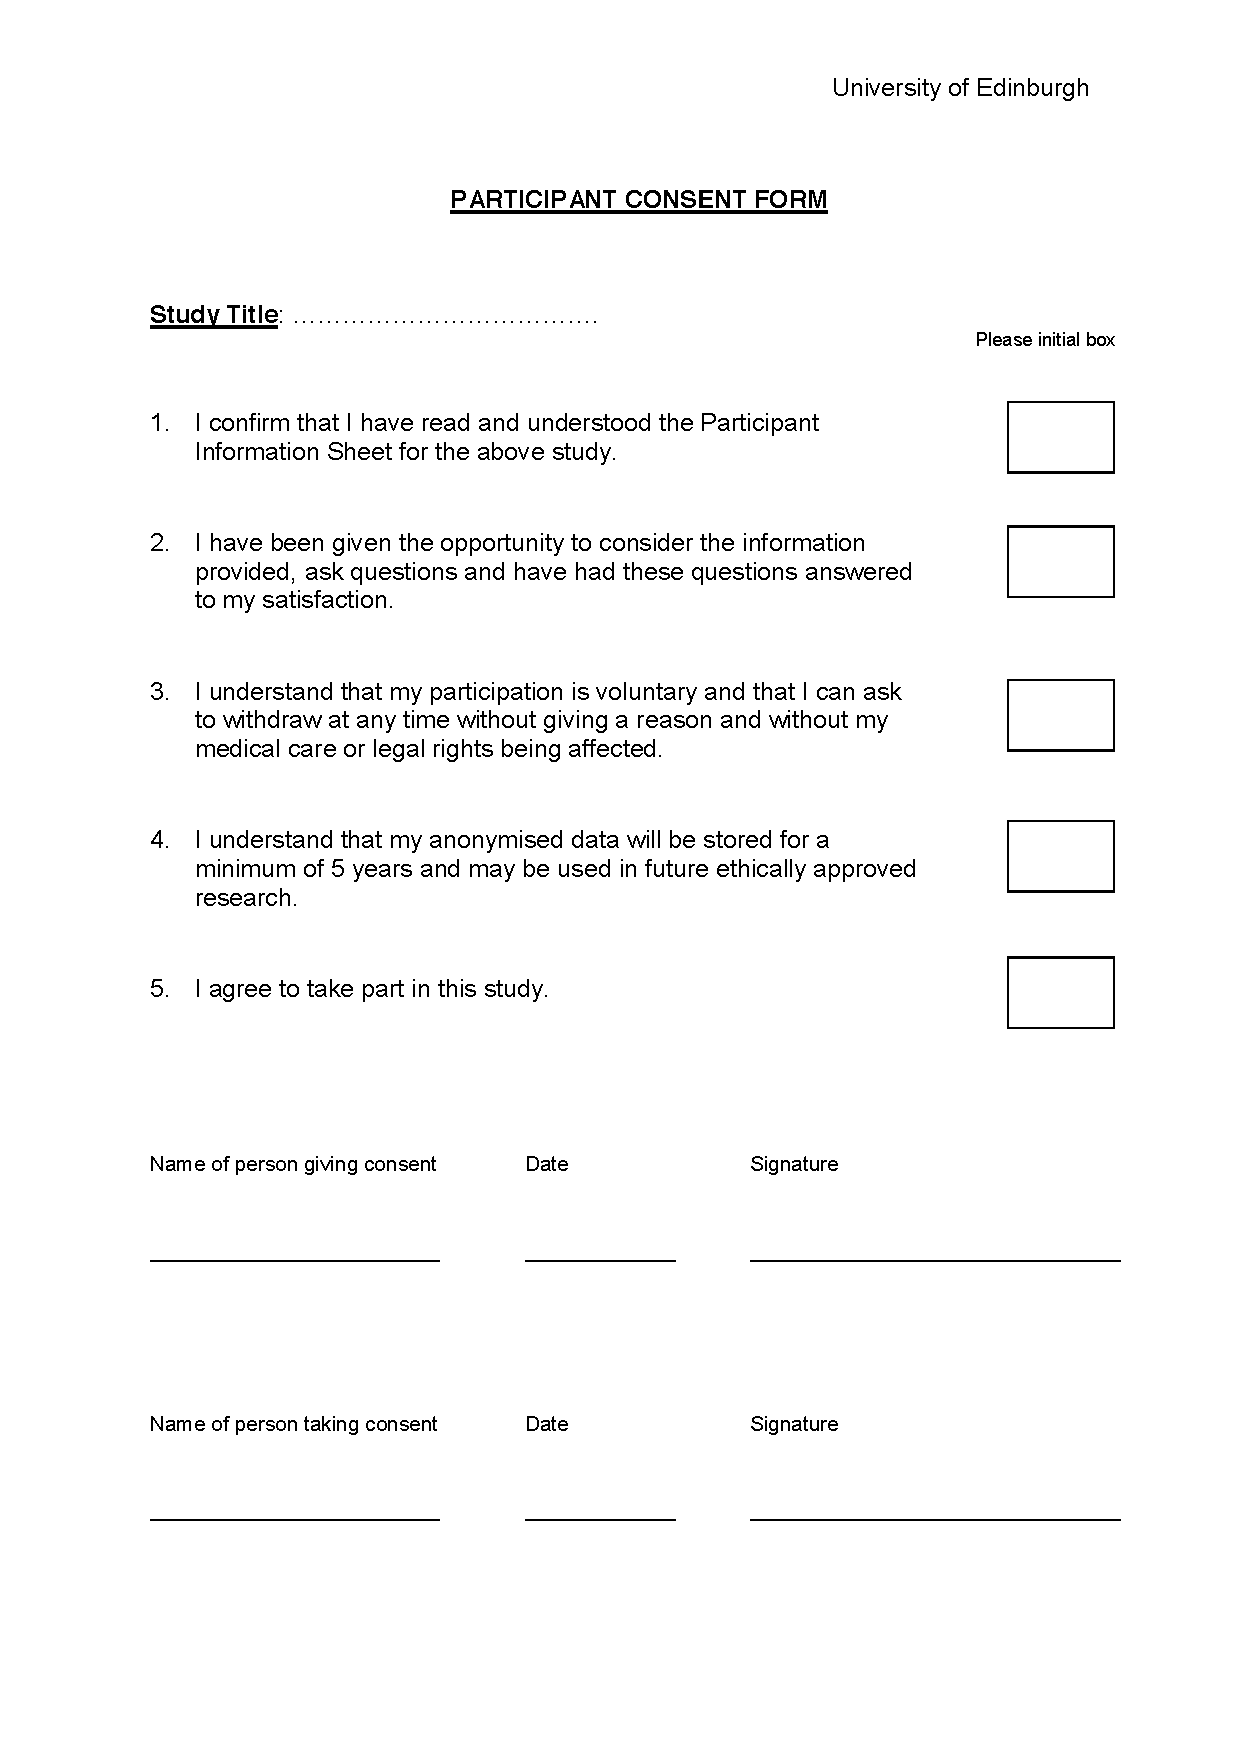
\includegraphics[width=\textwidth]{pdfs/consent}
\caption{Participant Consent Forms}
\label{consentform}
\end{figure}

\section{GDPR Course Certificate}
\label{sec:gdpr}

\begin{figure}[H]
\centering
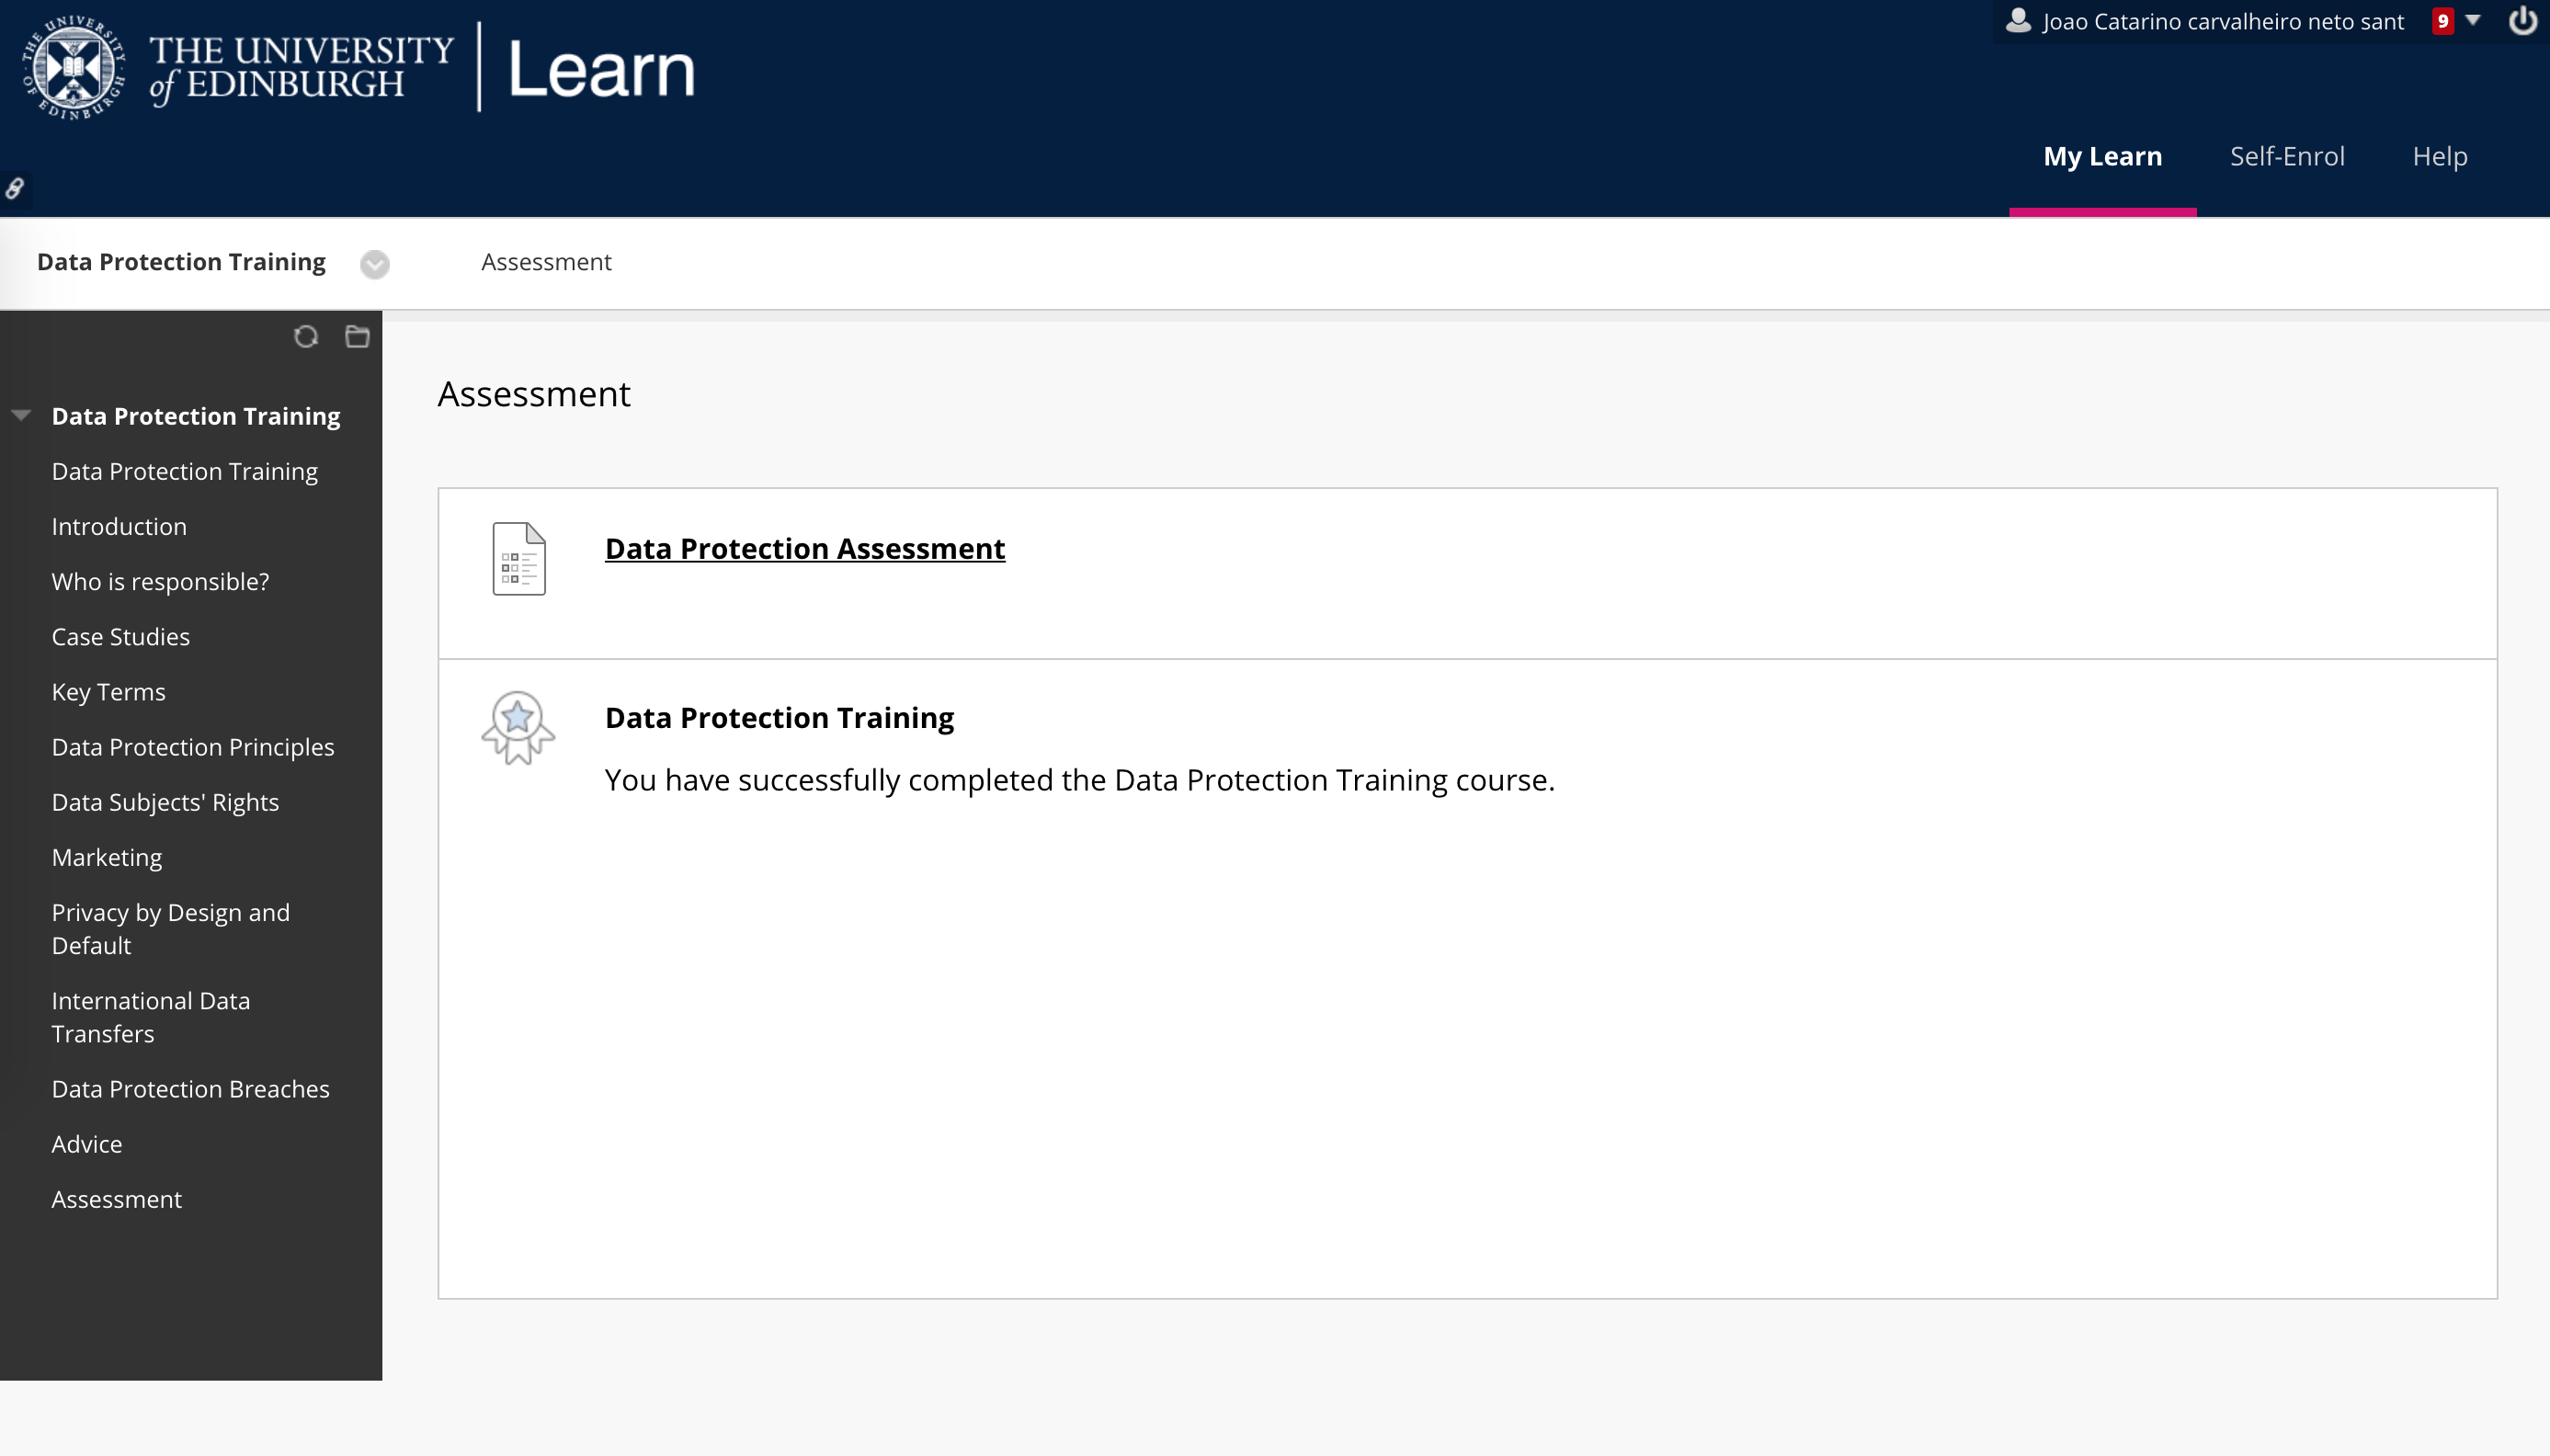
\includegraphics[width=\textwidth]{images/gdpr}
\caption{GDPR Course Certificate}
\label{consentform}
\end{figure}


\end{document}
